\chapter[Results and Statistical Model][Results and Statistical Model]{Results and Statistical Model} 
\label{chapter:results} 


The predicted number of background and signal events and the observed data for each of the signal regions (including sub-channels) are provided in Table~\ref{table:results}. We observe an excess of events in many of the 2$\ell$ and 3$\ell$ channels over the expected background. We provide a preliminary measurement of $\mu$, which is a ratio of the observed \tth\ production rate to the predicted SM production rate. We also interpret the results as a 95\% exclusion level on possible $\mu$ values. The statistical model used to make these measurements is discussed in depth below.


\begin{table}[h!]

\caption{Results in the 2$\ell$, 3$\ell$, and 4$\ell$ signal regions with flavor and jet sub-channels for 2$\ell$ and SFOS and non-SFOS sub-channels for 4$\ell$. The results included only statistical normalization }
\resizebox{1.0\textwidth}{!}{%
\begin{tabular}{|c|c|c|c|c|c|c|c|c|}
\hline
                & \tth              & \ttV               & \tZ               & VV                     & Fakes           & QMis            & Sum Background         & Data   \\
\hline
\textbf{2$\ell$ SS}    &  $6.74 \pm 0.61$ &   $31.00 \pm 4.03$ &  $1.59 \pm 0.21$ &        $5.30 \pm 2.65$ & $24.65 \pm 4.40$ & $4.87 \pm 1.08$ &       $67.41 \pm 6.62$ &    $98$\\
\hline
2ee4j     &  $0.45 \pm 0.04$ &    $2.86 \pm 0.37$ &  $0.20 \pm 0.03$ &        $0.89 \pm 0.45$ & $3.45 \pm 1.75$ & $1.82 \pm 0.34$ &        $9.22 \pm 1.87$ &    $9$\\

2ee5jincl     &  $0.74 \pm 0.07$ &    $2.46 \pm 0.32$ &  $0.13 \pm 0.02$ &        $0.60 \pm 0.30$ & $2.33 \pm 2.90$ & $1.11 \pm 0.56$ &        $6.63 \pm 2.99$ &     $10$\\

2em4j     &  $1.18 \pm 0.11$ &    $7.90 \pm 1.03$ &  $0.59 \pm 0.08$ &        $1.78 \pm 0.89$ & $12.33 \pm 1.55$ & $1.39 \pm 0.44$ &       $25.17 \pm 2.11$ &    $26$\\

2em5jincl     &  $2.17 \pm 0.20$ &    $7.21 \pm 0.94$ &  $0.29 \pm 0.04$ &        $0.64 \pm 0.32$ & $6.66 \pm 1.25$ & $0.85 \pm 0.43$ &       $17.84 \pm 1.75$ &    $22$\\

2mm4j     &  $0.76 \pm 0.07$ &    $5.63 \pm 0.73$ &  $0.23 \pm 0.03$ &        $0.56 \pm 0.28$ & $6.32 \pm 1.73$ &  0    & $12.62 \pm 1.90$ &    $20$\\
2mm5jincl     &  $1.44 \pm 0.13$ &    $4.94 \pm 0.64$ &  $0.14 \pm 0.02$ &        $0.83 \pm 0.42$ & $2.89 \pm 0.96$ & 0&       $8.58 \pm 1.23$ &    $11$\\
\hline
\textbf{3$\ell$}    &  $2.39 \pm 0.21$ &    $6.56 \pm 0.85$ &  $0.58 \pm 0.07$ &        $1.81 \pm 0.91$ & $2.62 \pm 0.50$ &  0&     $11.57 \pm 1.34$ &    $18$\\
\hline
\textbf{4$\ell$}    &  $0.20 \pm 0.02$ &    $0.45 \pm 0.06$ &  $0.05 \pm 0.01$ &        $0.05 \pm 0.01$ &      $0.03 \pm 0.01$ & 0&                 $0.57 \pm 0.06$ &     $1$\\
\hline
\end{tabular}%
}
\label{table:results}
\end{table}


\section{Results in Signal Regions}
Plots of event variables are shown in Figures \ref{figure:results_2l_event} - \ref{figure:results_2l_jet} for the 2$\ell$ SS signal region and Figures \ref{figure:results_3l_event} - \ref{figure:results_3l_jet} for the 3 $\ell$ signal. The 4 $\ell$ regions have too few events to be informative.  Likewise, the statistics of the backgrounds models are too poor in the sub-channels of the  2$\ell$ signal region. The results are shown instead for the inclusive 2$\ell$ signal region. The charge misidentification and fake backgrounds take their normalizations from the measurements in Chapter~\ref{chapter:background}, while their shapes are directly from MC. The plots show the combined statistical uncertainties and systematic uncertainties from theory and background normalization as well as experimental and detector effects. 

\begin{figure}[!htbp]
  \begin{minipage}[h]{0.4\textwidth}
    \centering 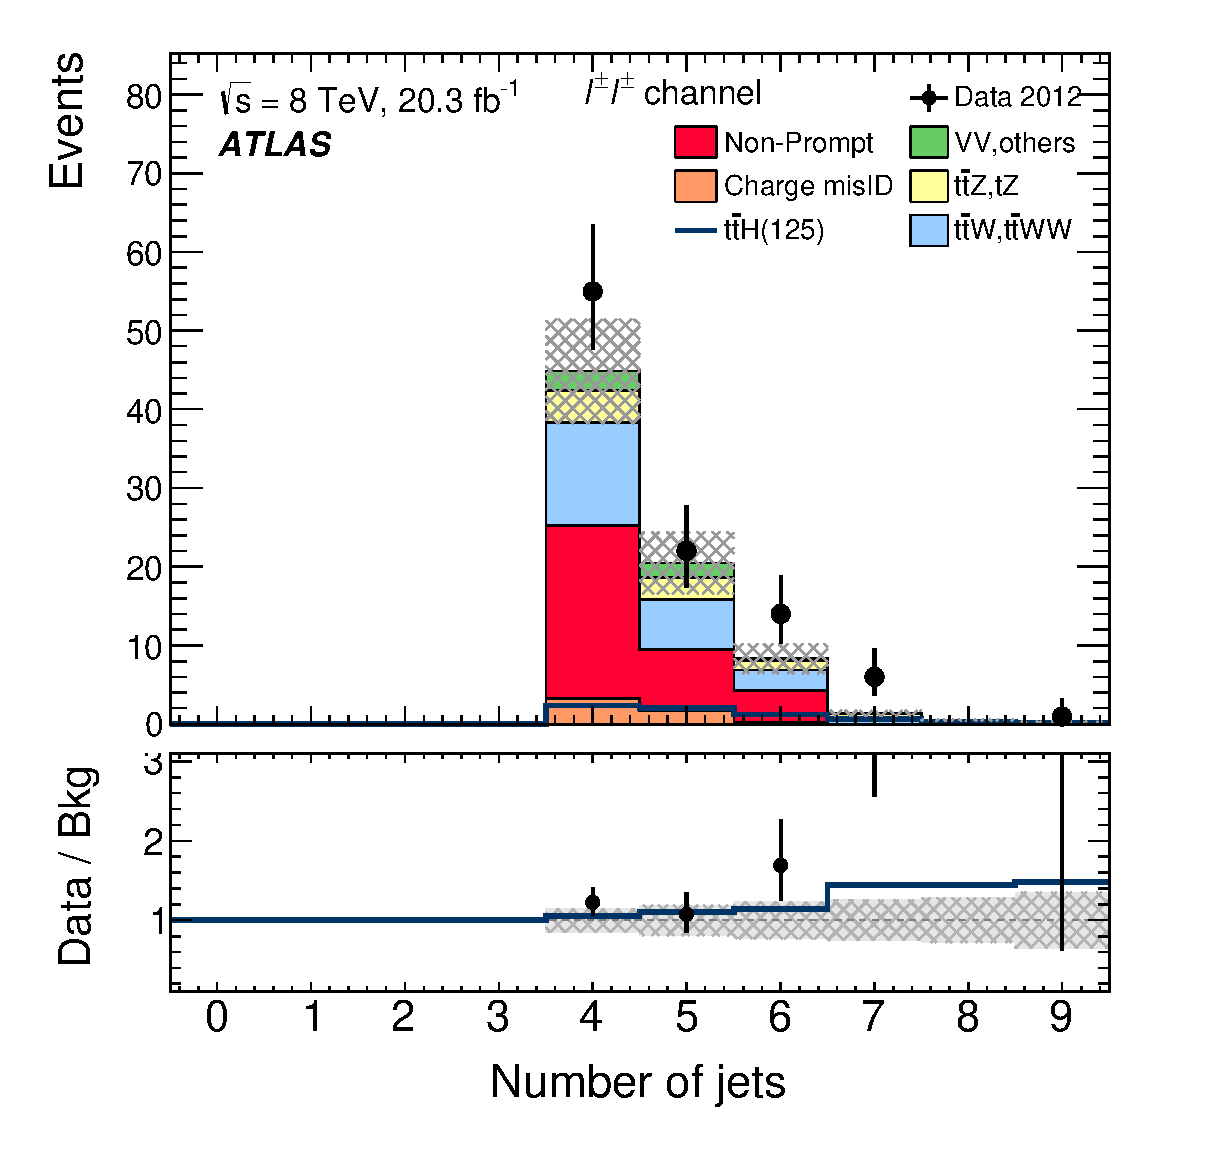
\includegraphics[width=\textwidth]{figs/results/results_new/2lep_SR_NJet}
  \end{minipage}\hfill
  \begin{minipage}[h]{0.4\textwidth}
    \centering 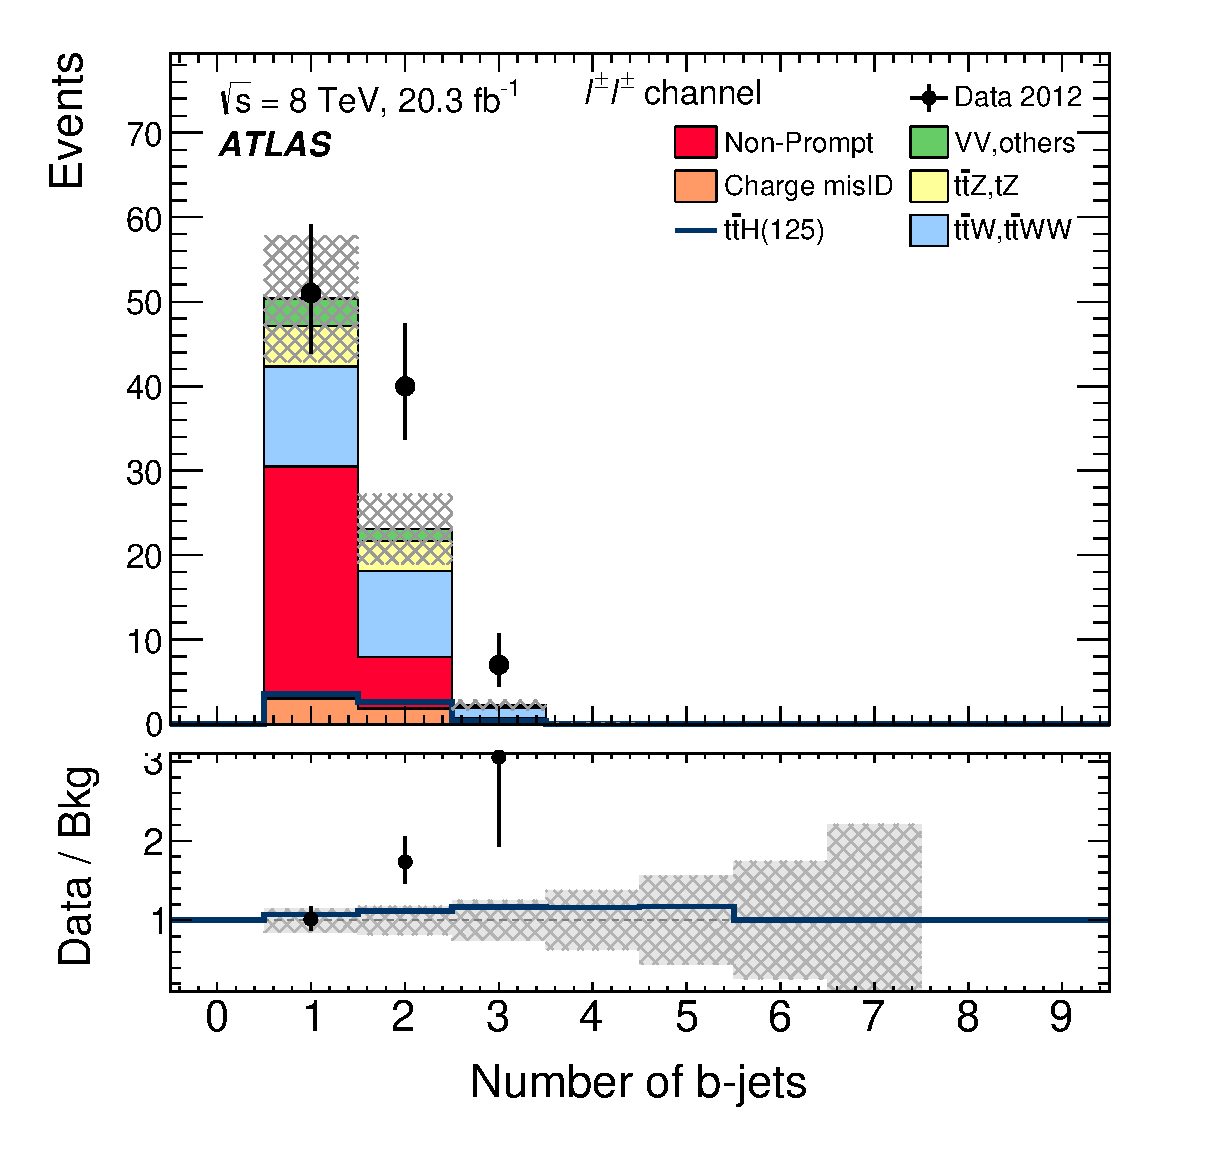
\includegraphics[width=\textwidth]{figs/results/results_new/2lep_SR_NJetBTag}
  \end{minipage}\hfill
  \begin{minipage}[h]{0.4\textwidth}
    \centering 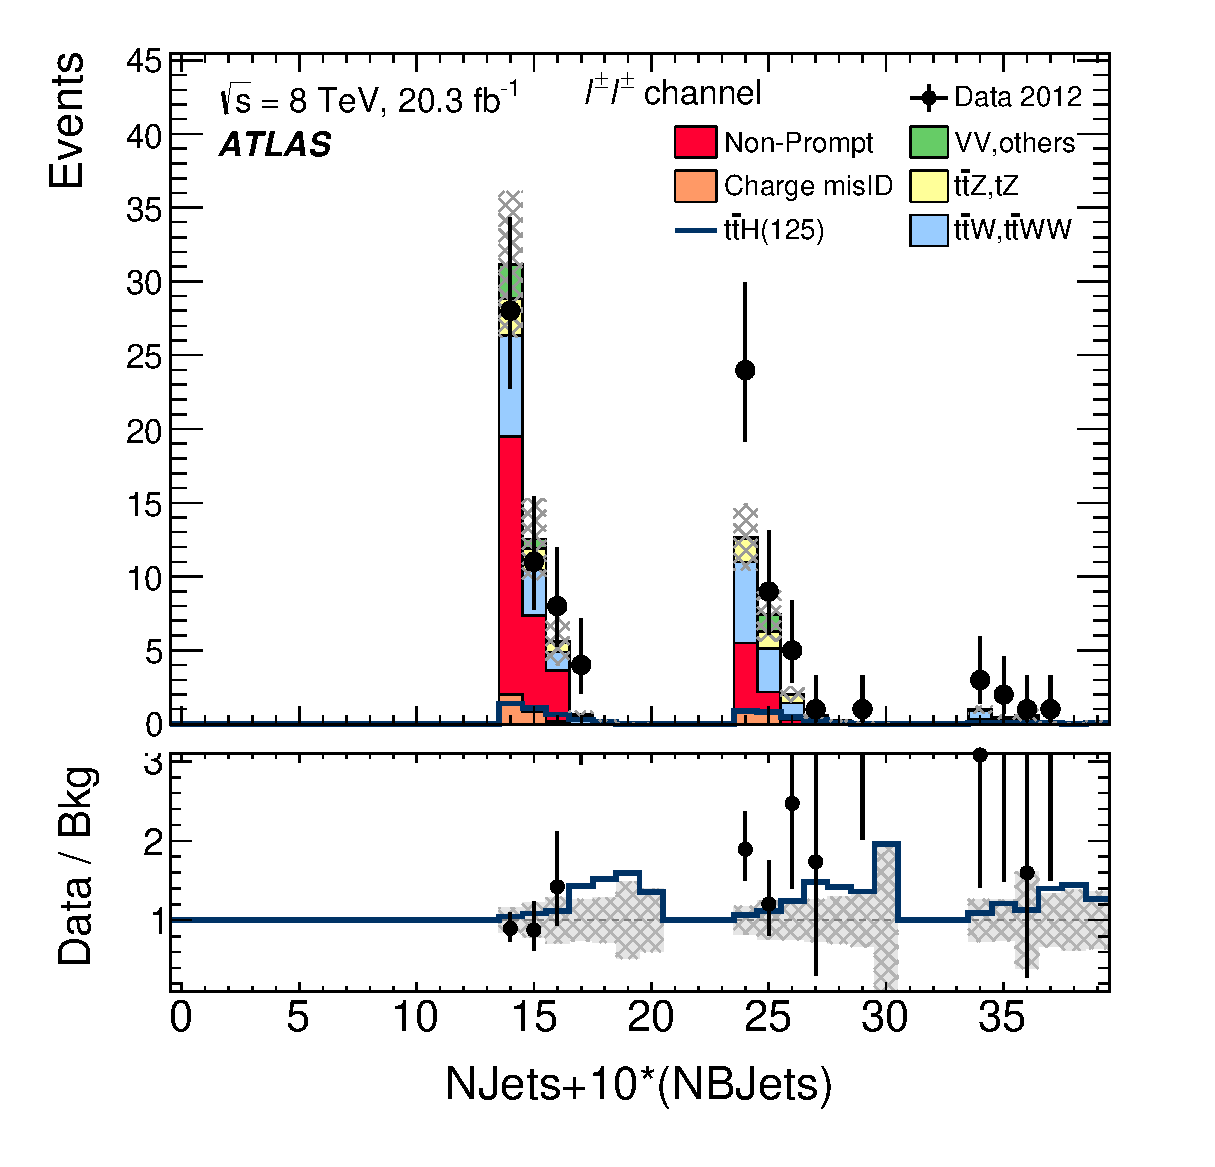
\includegraphics[width=\textwidth]{figs/results/results_new/2lep_SR_NJetCombined}
  \end{minipage}\hfill
  \begin{minipage}[h]{0.4\textwidth}
    \centering 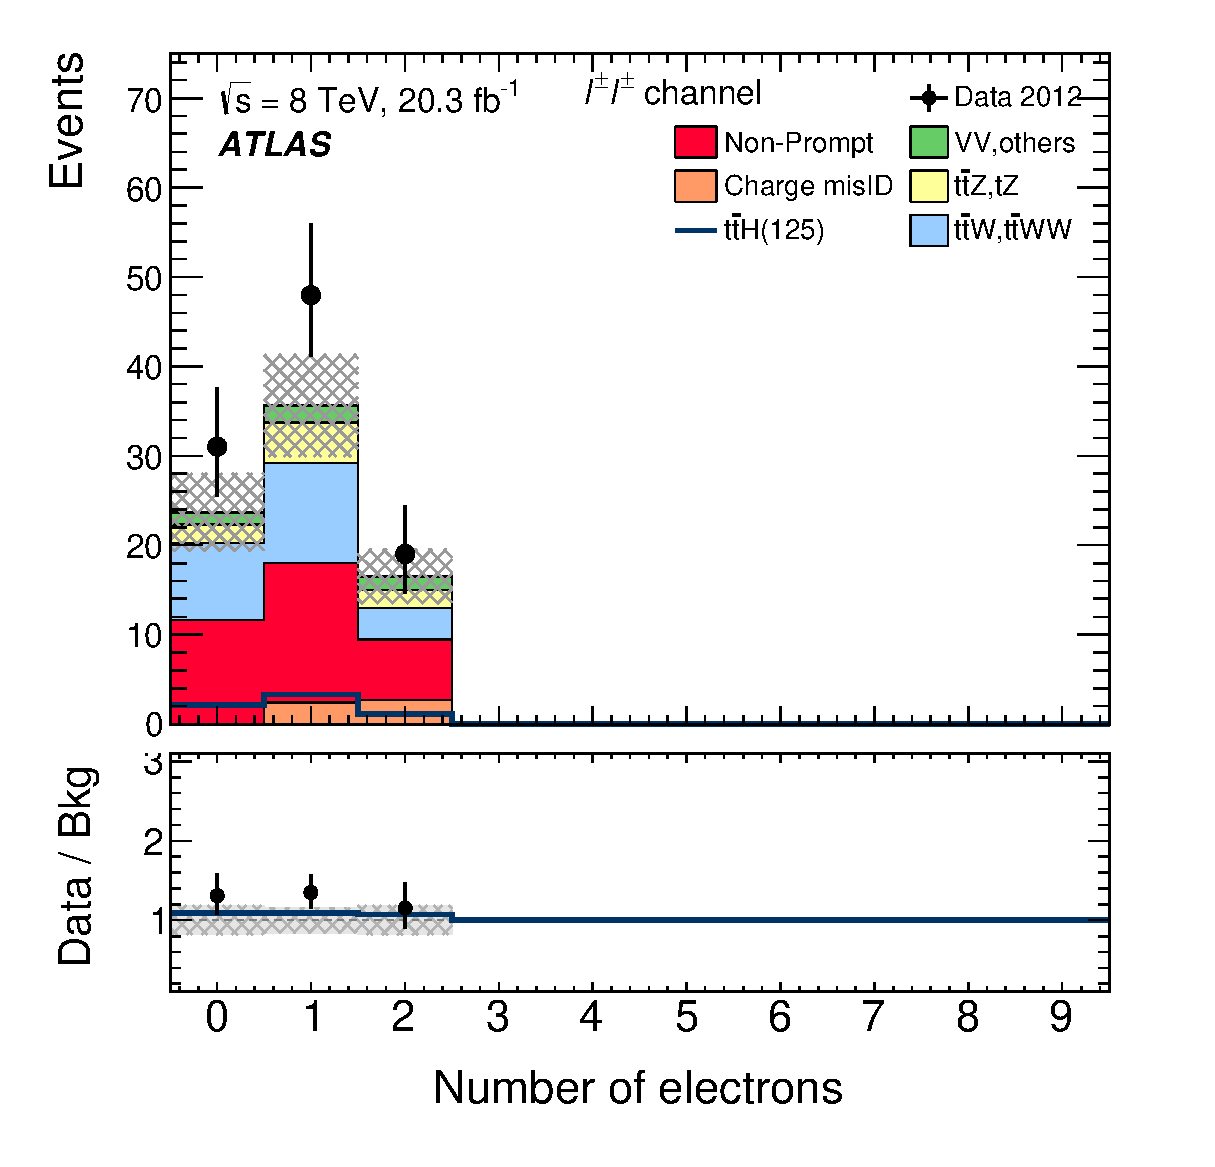
\includegraphics[width=\textwidth]{figs/results/results_new/2lep_SR_NElec}
  \end{minipage}\hfill
  \begin{minipage}[h]{0.4\textwidth}
    \centering 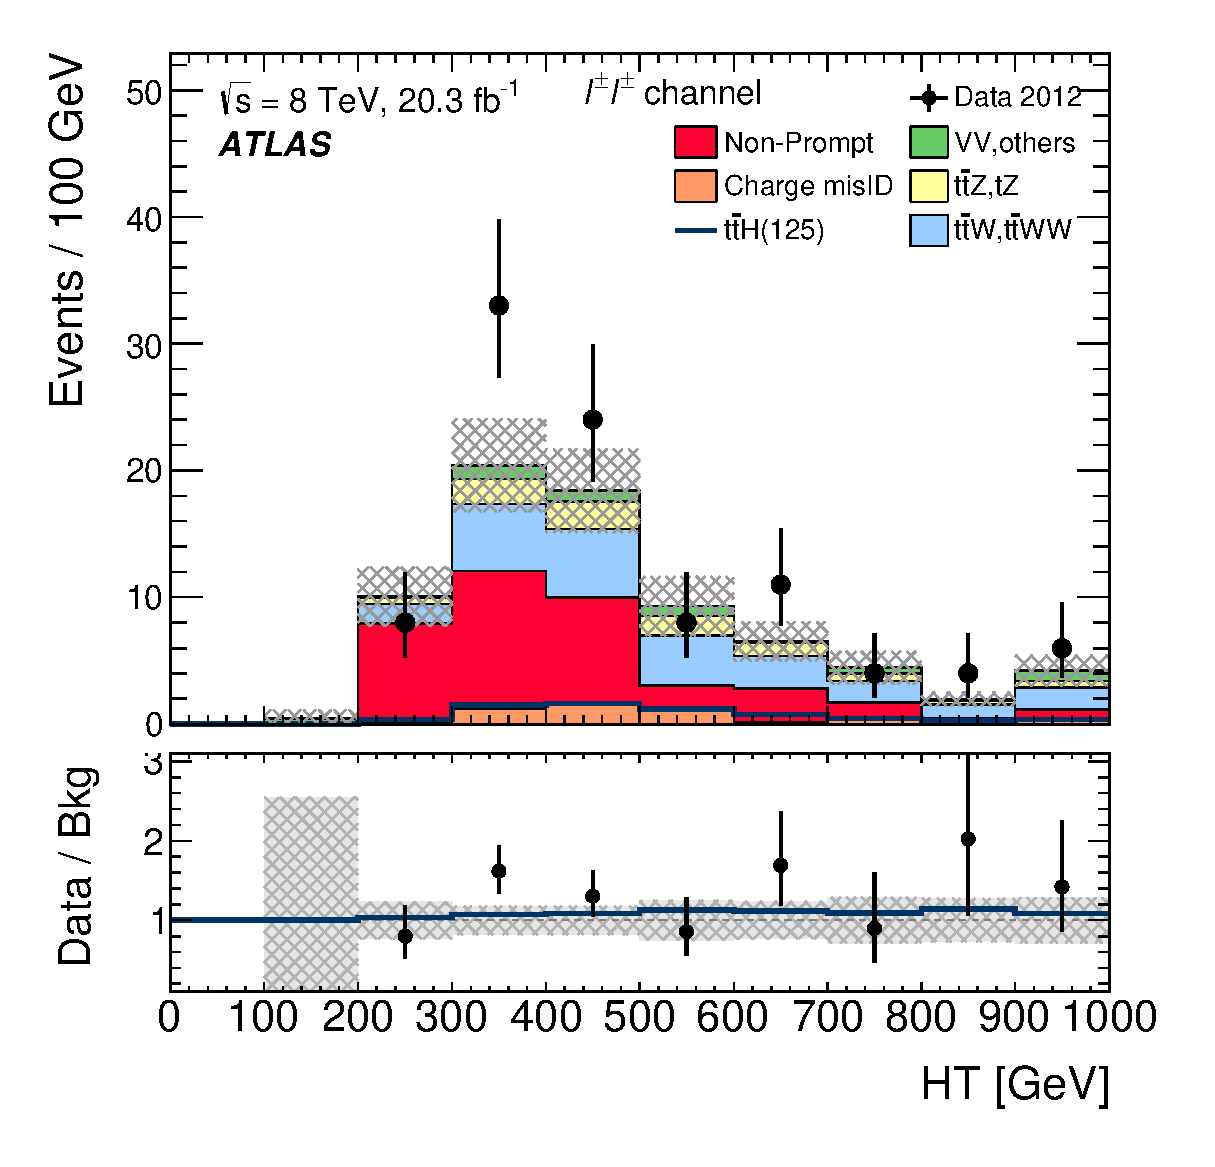
\includegraphics[width=\textwidth]{figs/results/results_new/2lep_SR_HT}
  \end{minipage}\hfill
  \begin{minipage}[h]{0.4\textwidth}
    \centering 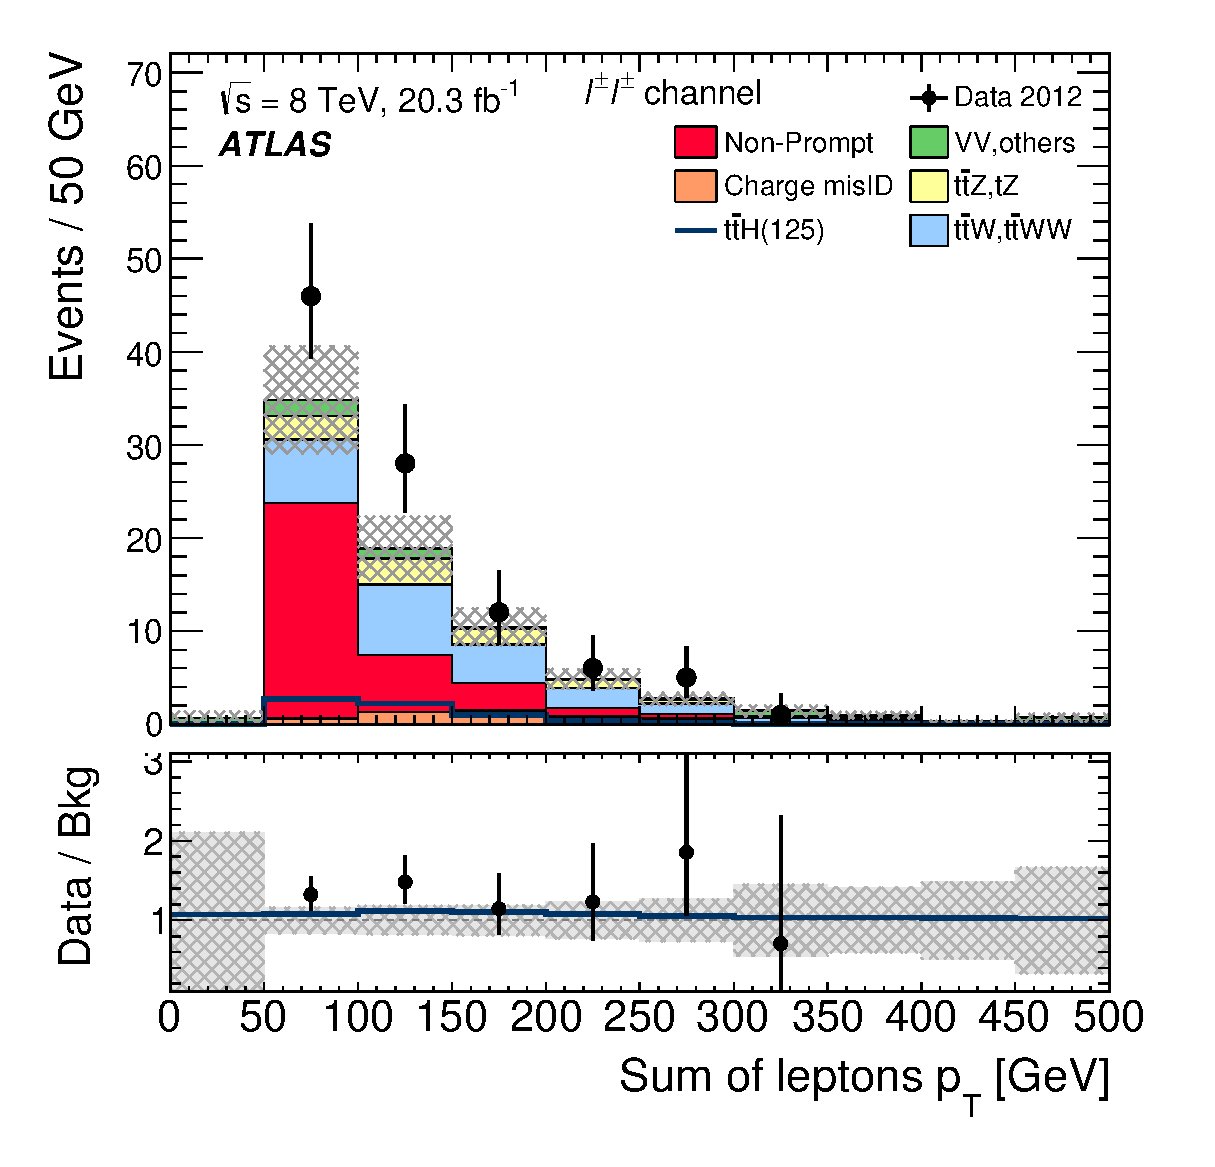
\includegraphics[width=\textwidth]{figs/results/results_new/2lep_SR_SumPtLep}
  \end{minipage}\hfill
  \caption{Distributions for combined 2-lepton signal region without hadronic taus.
    Jet and b-tagged jet multiplicities (top row);
    10*n(b-tags)+n(jets) and electron multiplicity (middle tow);
    scalar sum of the \pt of selected leptons and jets in the event (bottom left) and only of leptons (bottom right).
}
  \label{figure:results_2l_event}
\end{figure} 
%
\begin{figure}[!htbp]
  \begin{minipage}[h]{0.4\textwidth}
    \centering 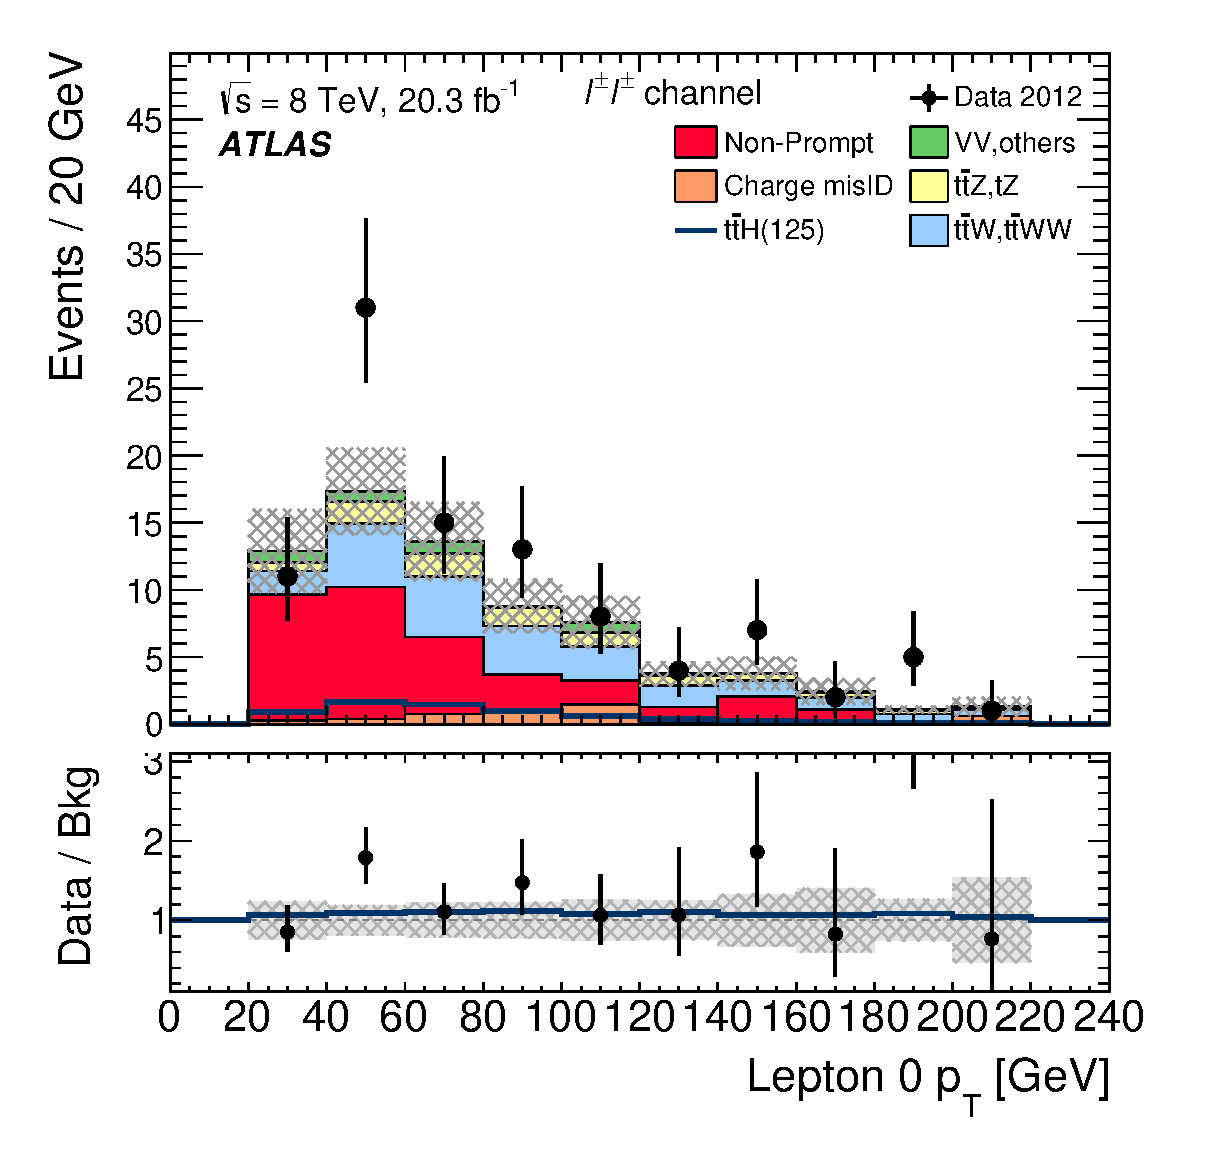
\includegraphics[width=\textwidth]{figs/results/results_new/2lep_SR_Lep0Pt}
  \end{minipage}\hfill
  \begin{minipage}[h]{0.4\textwidth}
    \centering 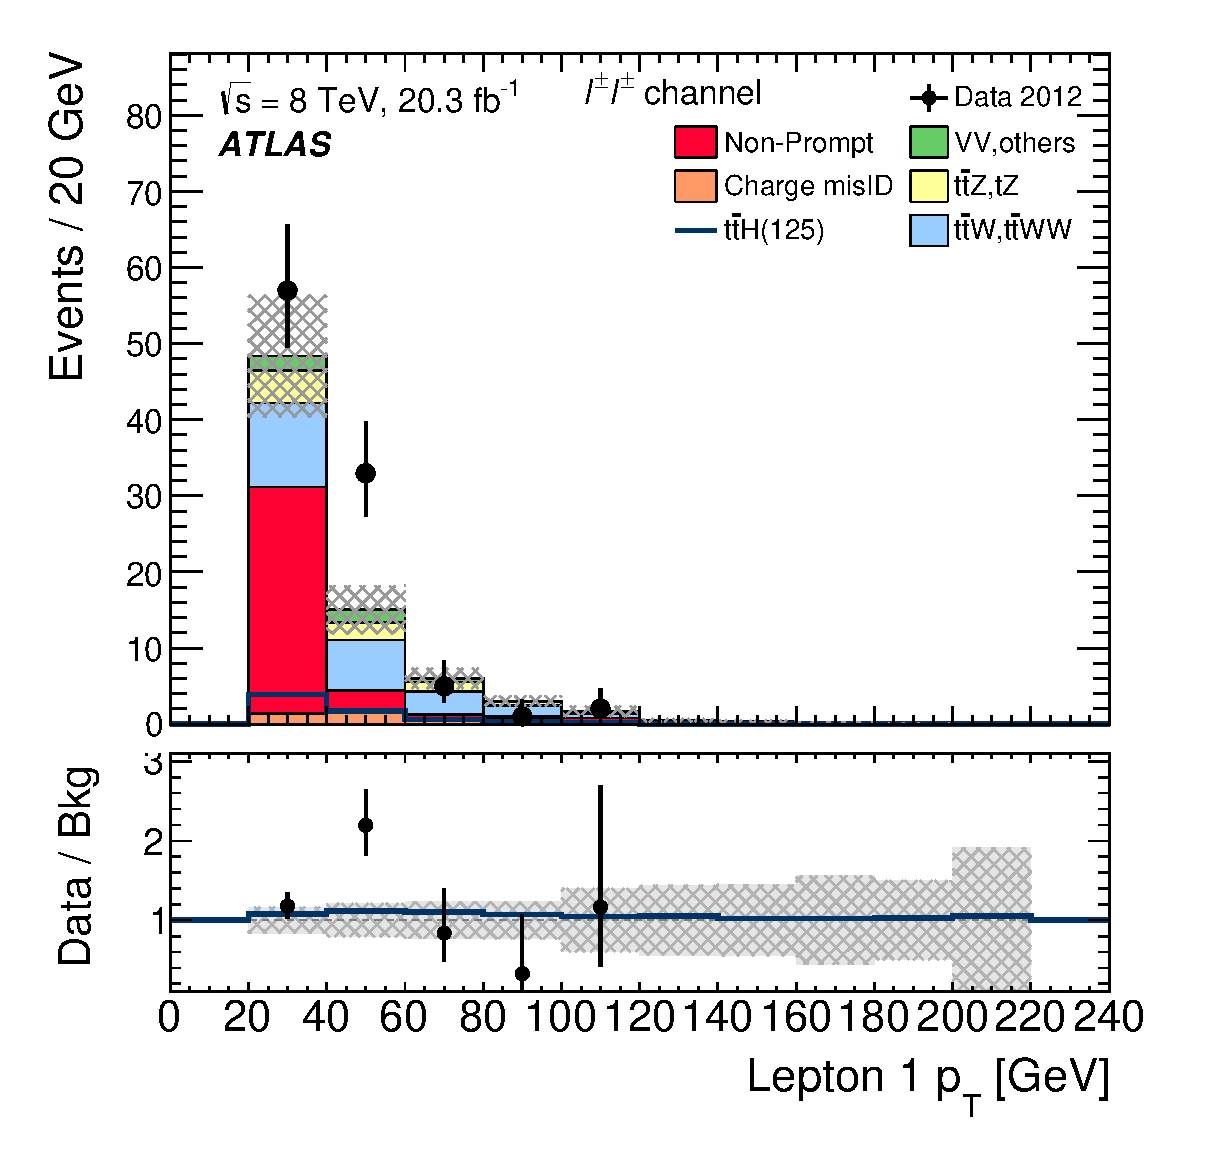
\includegraphics[width=\textwidth]{figs/results/results_new/2lep_SR_Lep1Pt}
  \end{minipage}\hfill
  \begin{minipage}[h]{0.4\textwidth}
    \centering 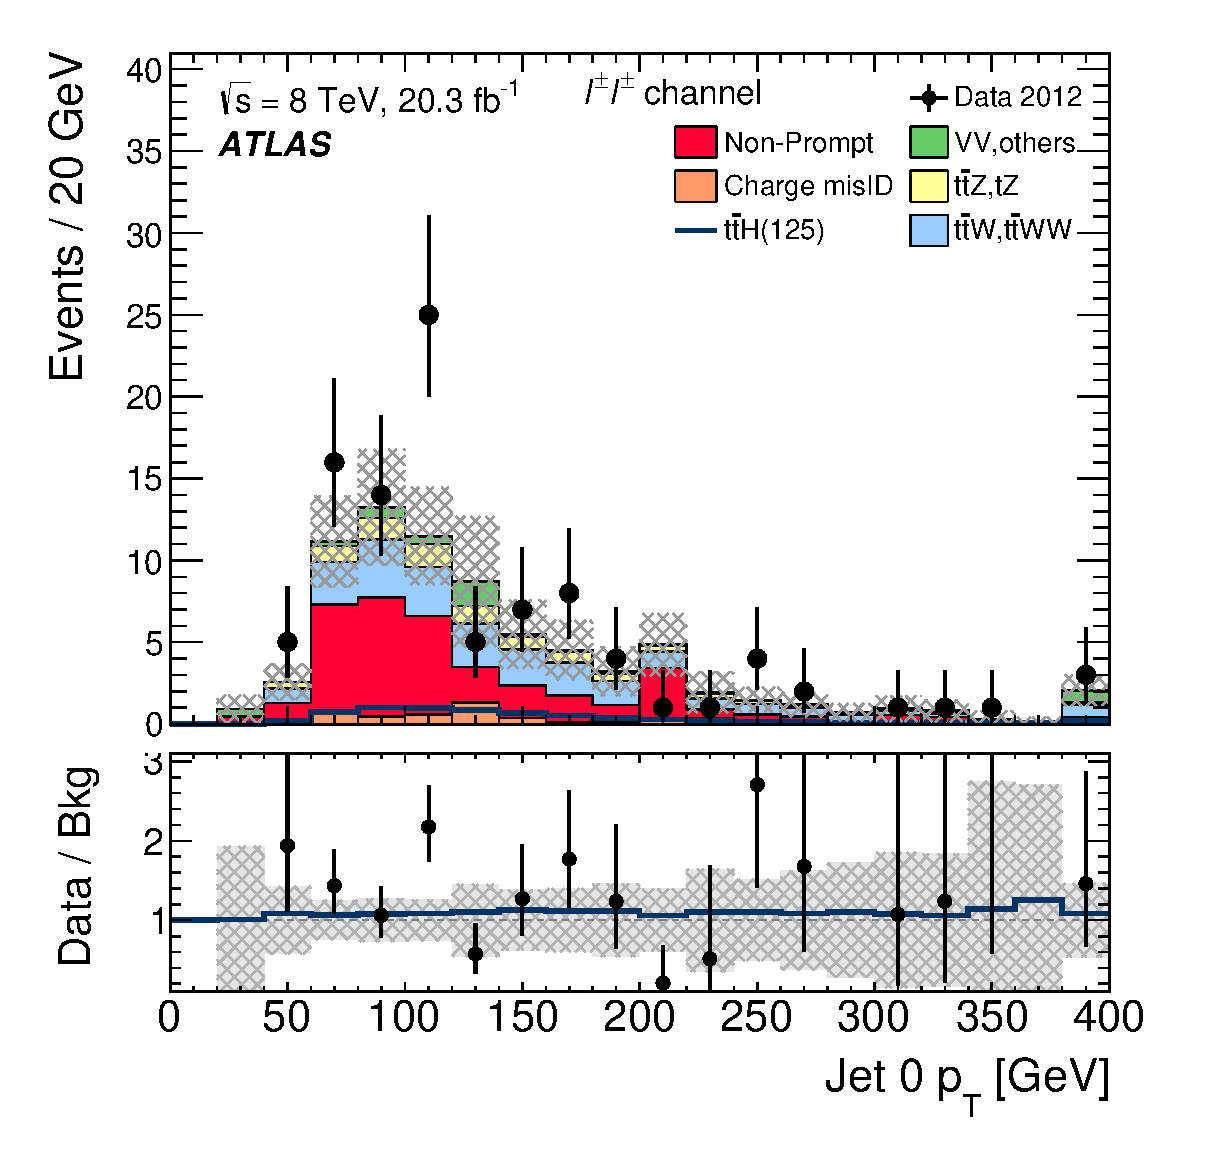
\includegraphics[width=\textwidth]{figs/results/results_new/2lep_SR_jet00_Pt}
  \end{minipage}\hfill
  \begin{minipage}[h]{0.4\textwidth}
    \centering 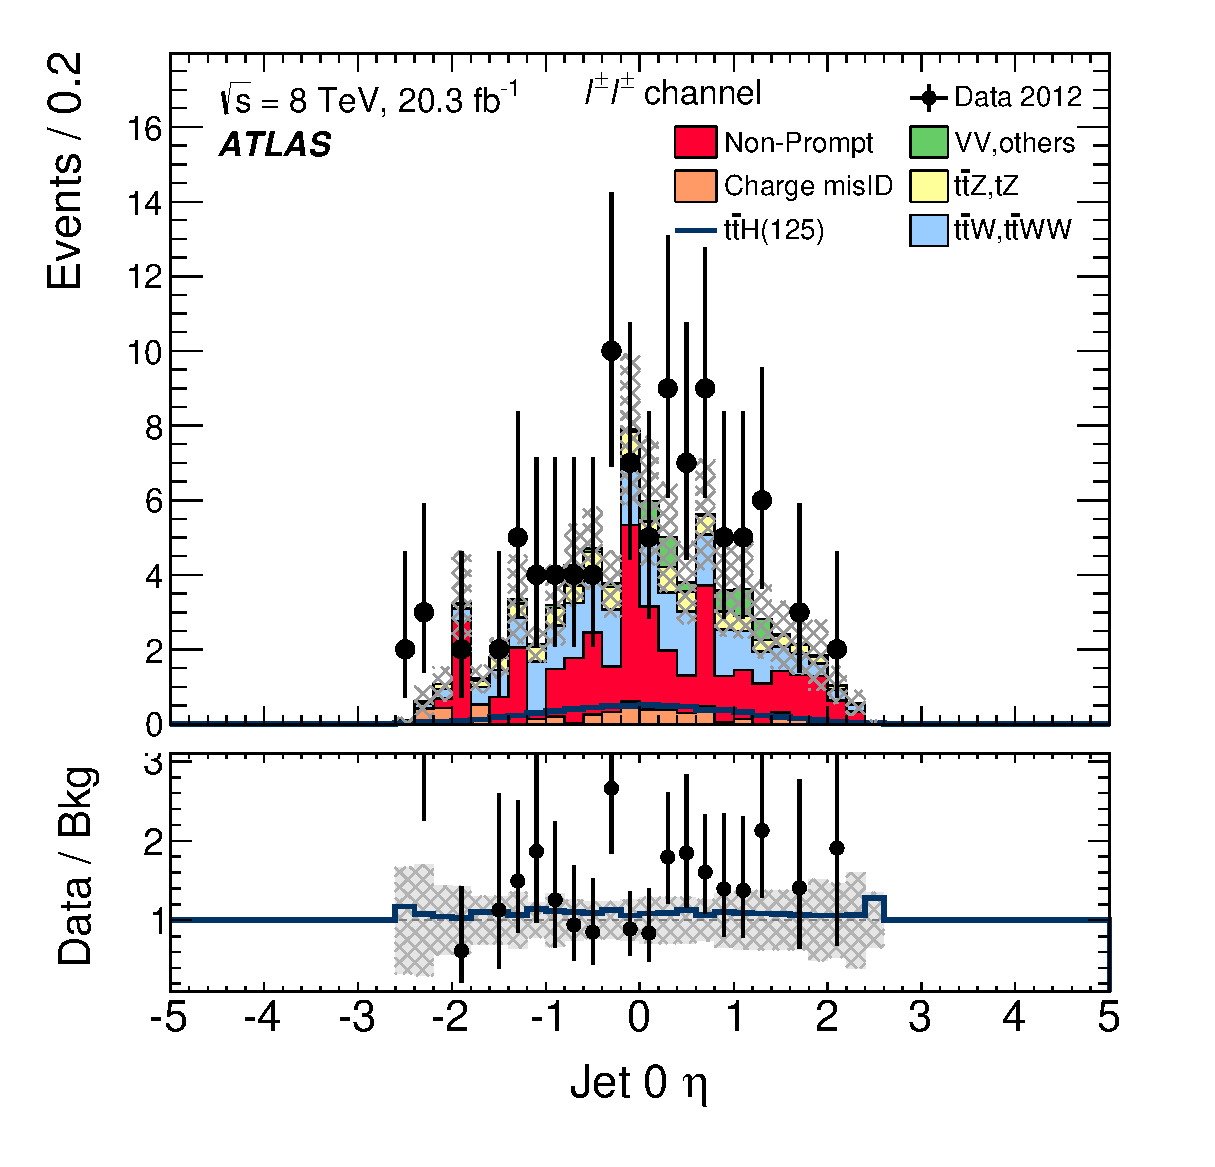
\includegraphics[width=\textwidth]{figs/results/results_new/2lep_SR_jet00_Eta}
  \end{minipage}\hfill
  \begin{minipage}[h]{0.4\textwidth}
    \centering 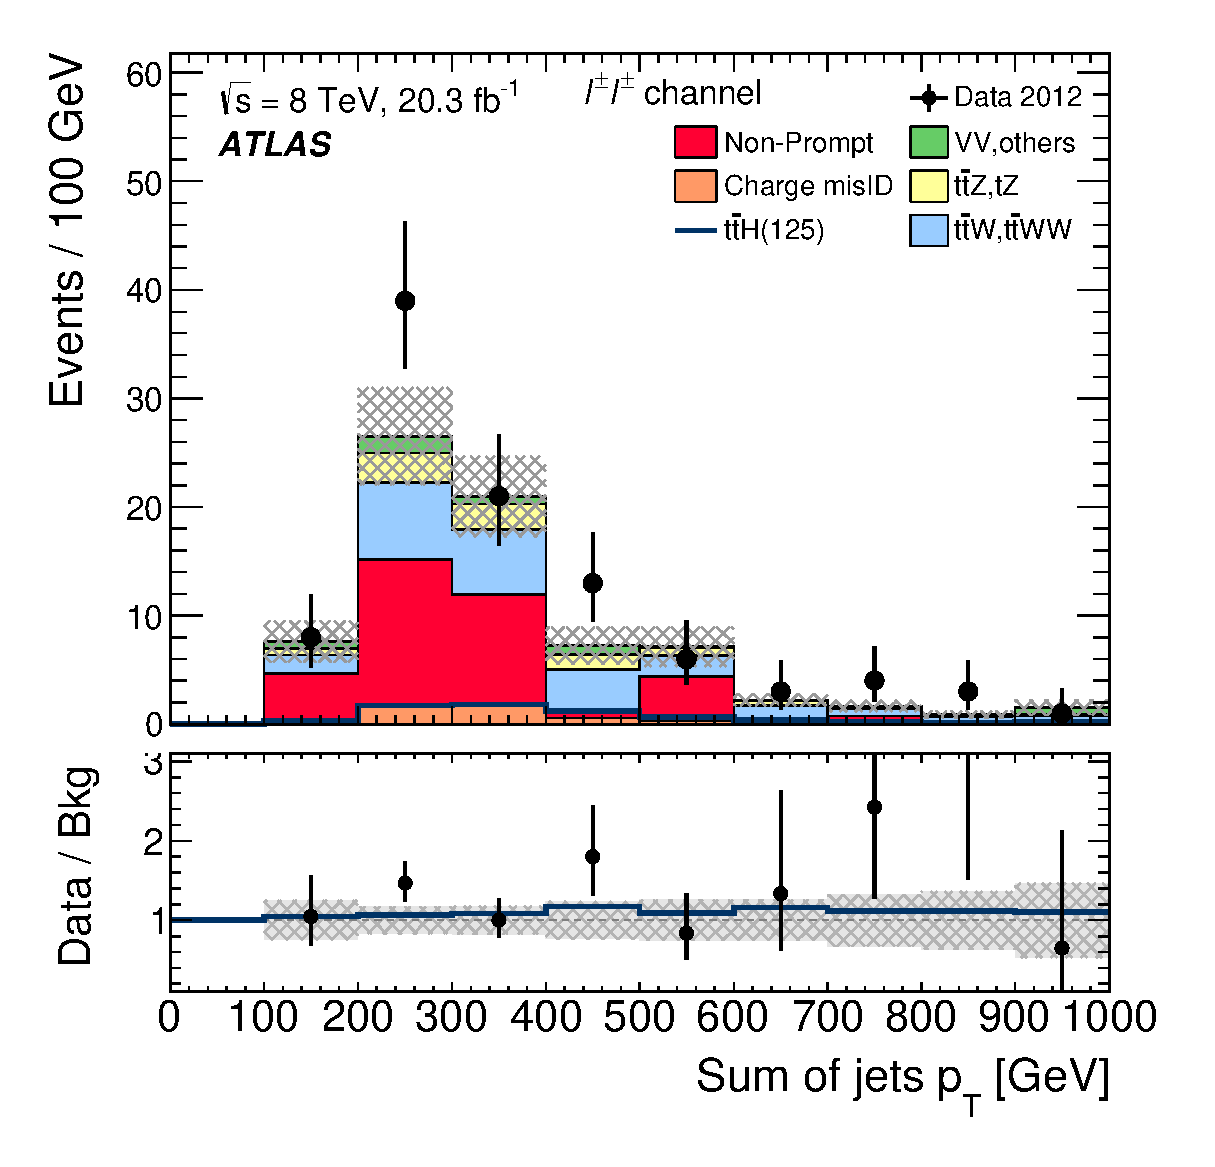
\includegraphics[width=\textwidth]{figs/results/results_new/2lep_SR_SumPtJet}
  \end{minipage}\hfill
  \begin{minipage}[h]{0.4\textwidth}
    \centering 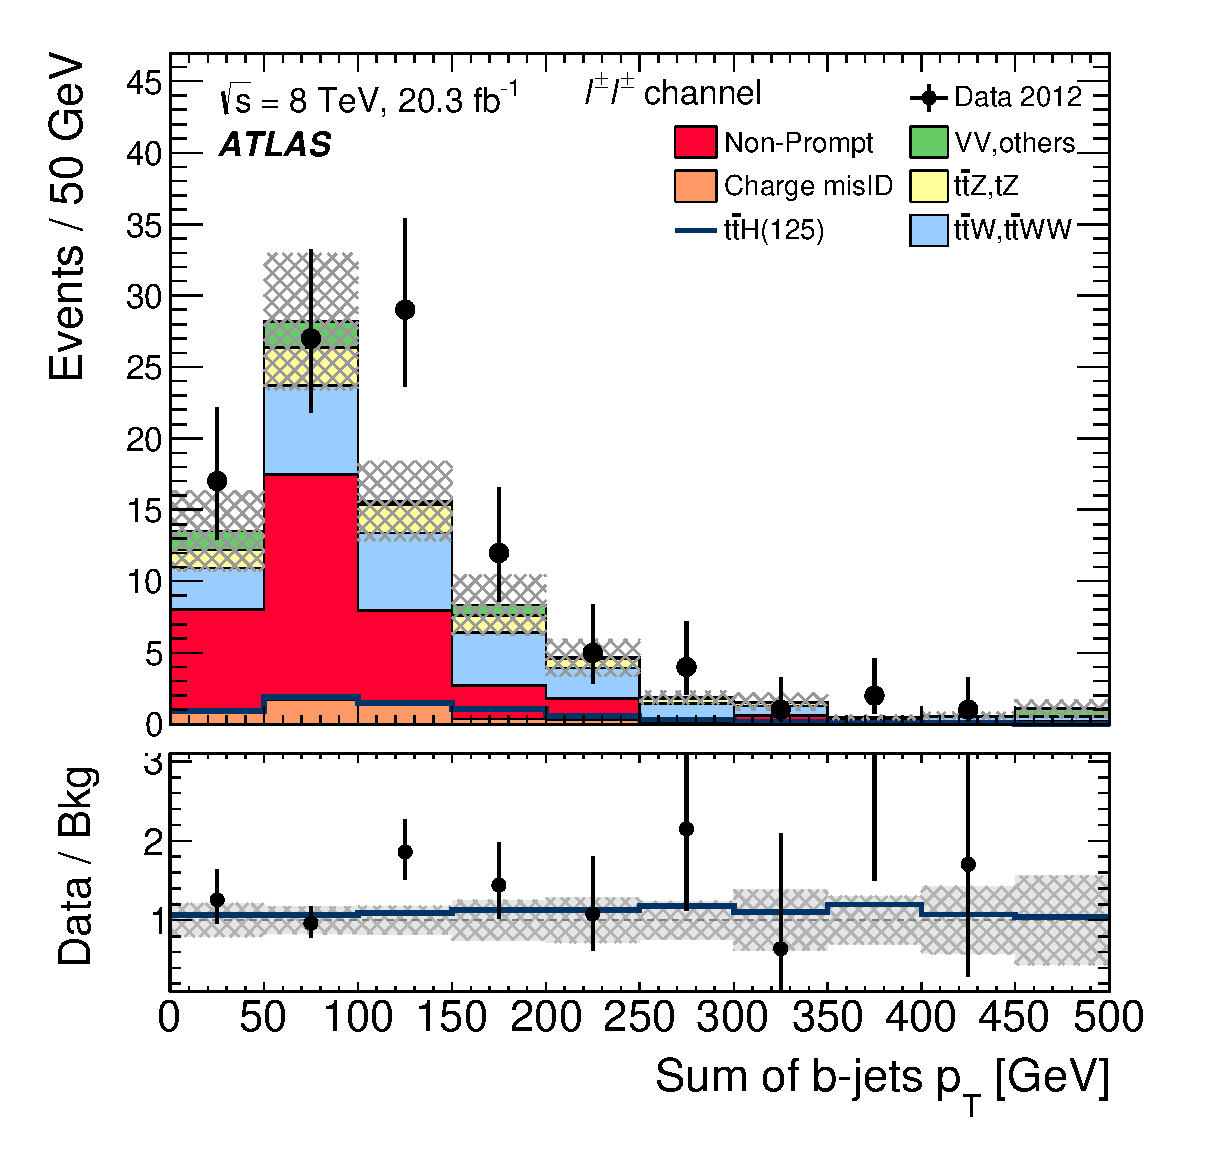
\includegraphics[width=\textwidth]{figs/results/results_new/2lep_SR_SumPtBJet}
  \end{minipage}\hfill
  \caption{Distributions for combined 2-lepton signal region without hadronic taus.
    Leading and sub-leading lepton \pt (top); leading jet \pt and $\eta$ (middle right); 
    scalar sum of the \pt of selected jets in the event (bottom left) and only of b-tagged jets (bottom right).}
  \label{figure:results_2l_jet}
\end{figure} 

\begin{figure}[!htbp]
  \begin{minipage}[h]{0.4\textwidth}
    \centering 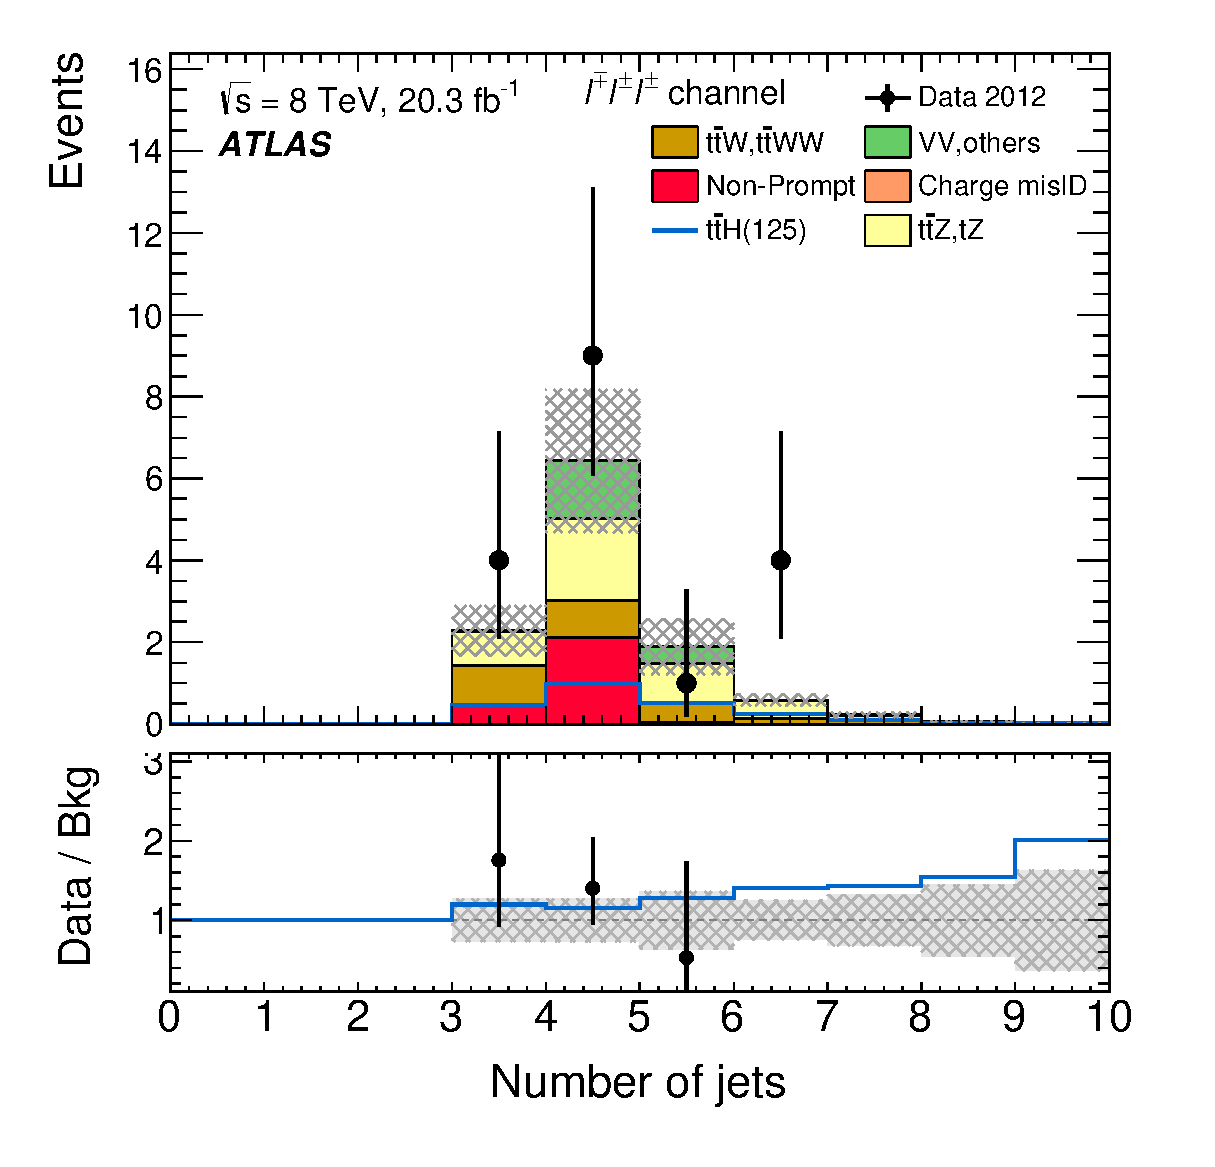
\includegraphics[width=\textwidth]{figs/results/results_new/3lep_SR_NJet}
  \end{minipage}\hfill
  \begin{minipage}[h]{0.4\textwidth}
    \centering 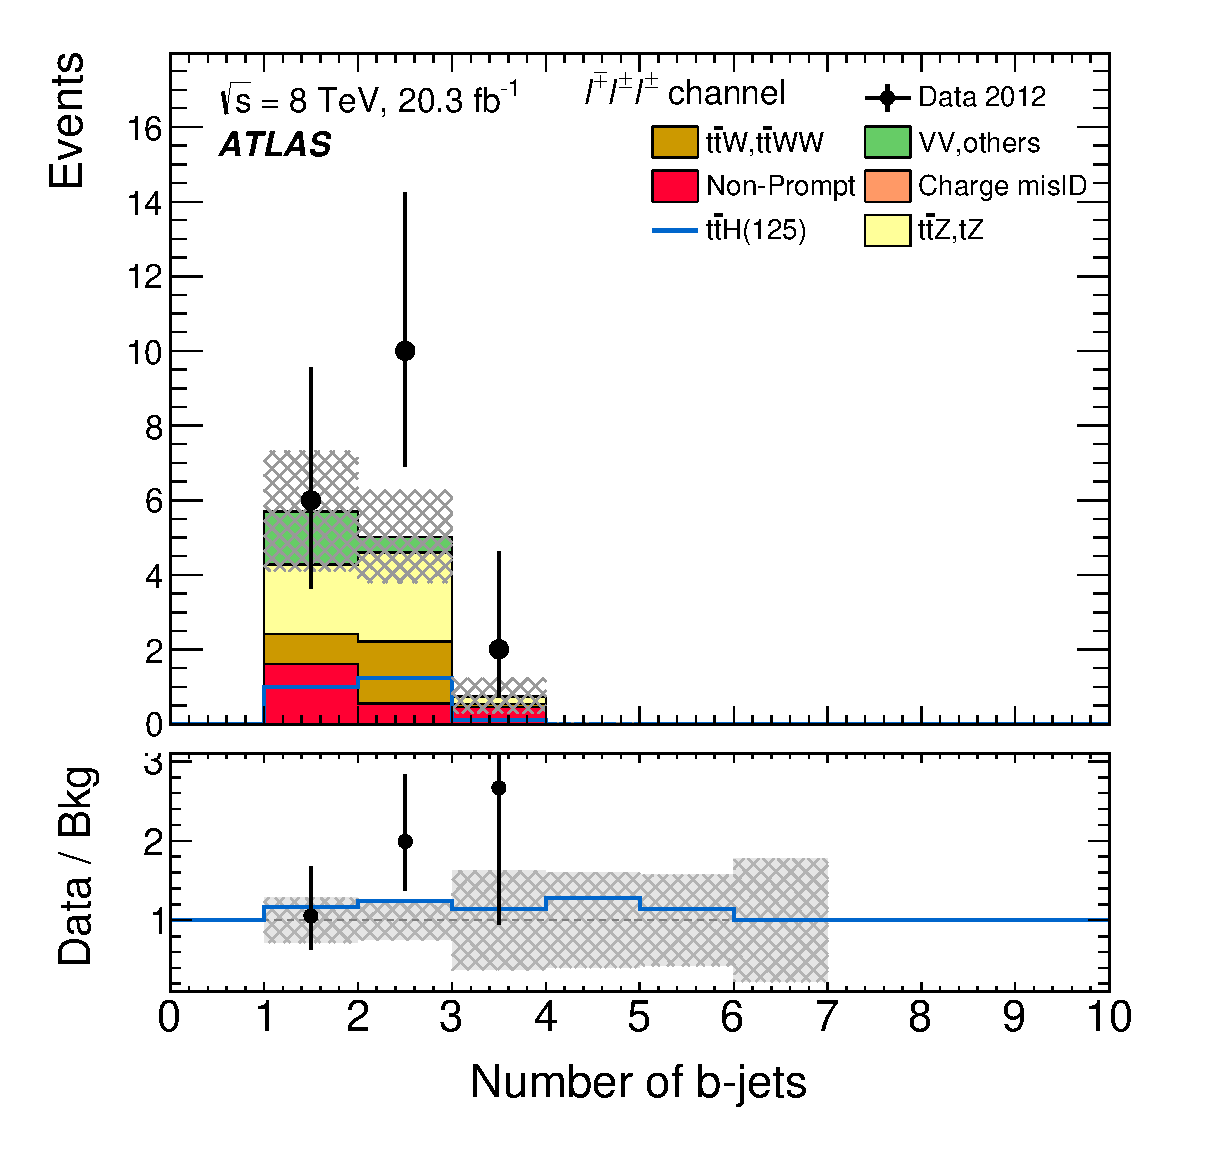
\includegraphics[width=\textwidth]{figs/results/results_new/3lep_SR_NJetBTag}
  \end{minipage}\hfill
  \begin{minipage}[h]{0.4\textwidth}
    \centering 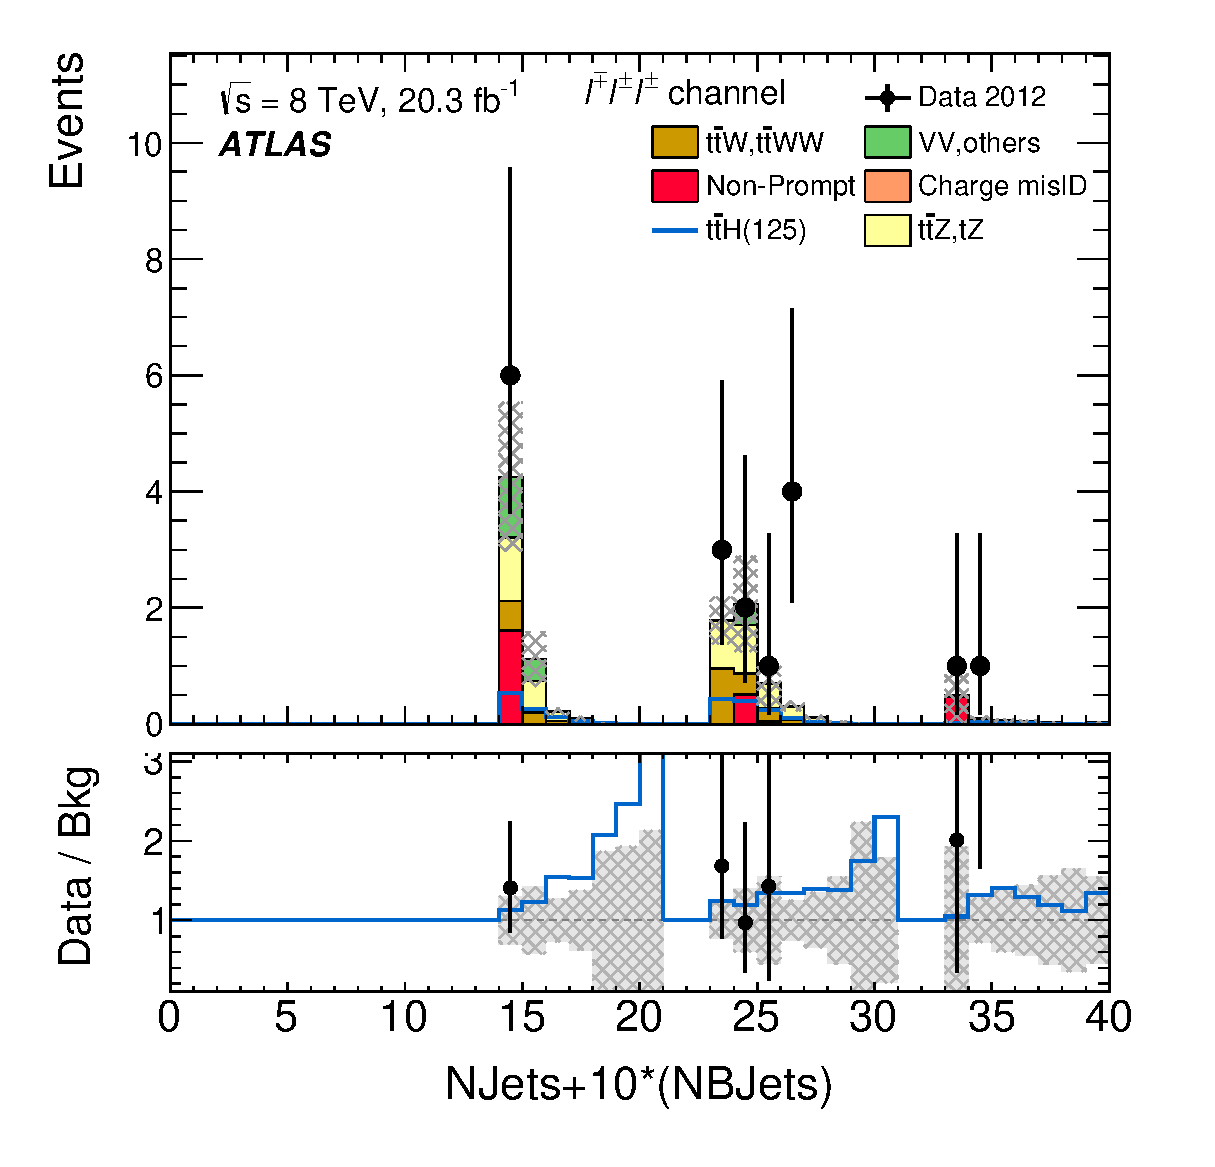
\includegraphics[width=\textwidth]{figs/results/results_new/3lep_SR_NJetCombined}
  \end{minipage}\hfill
  \begin{minipage}[h]{0.4\textwidth}
    \centering 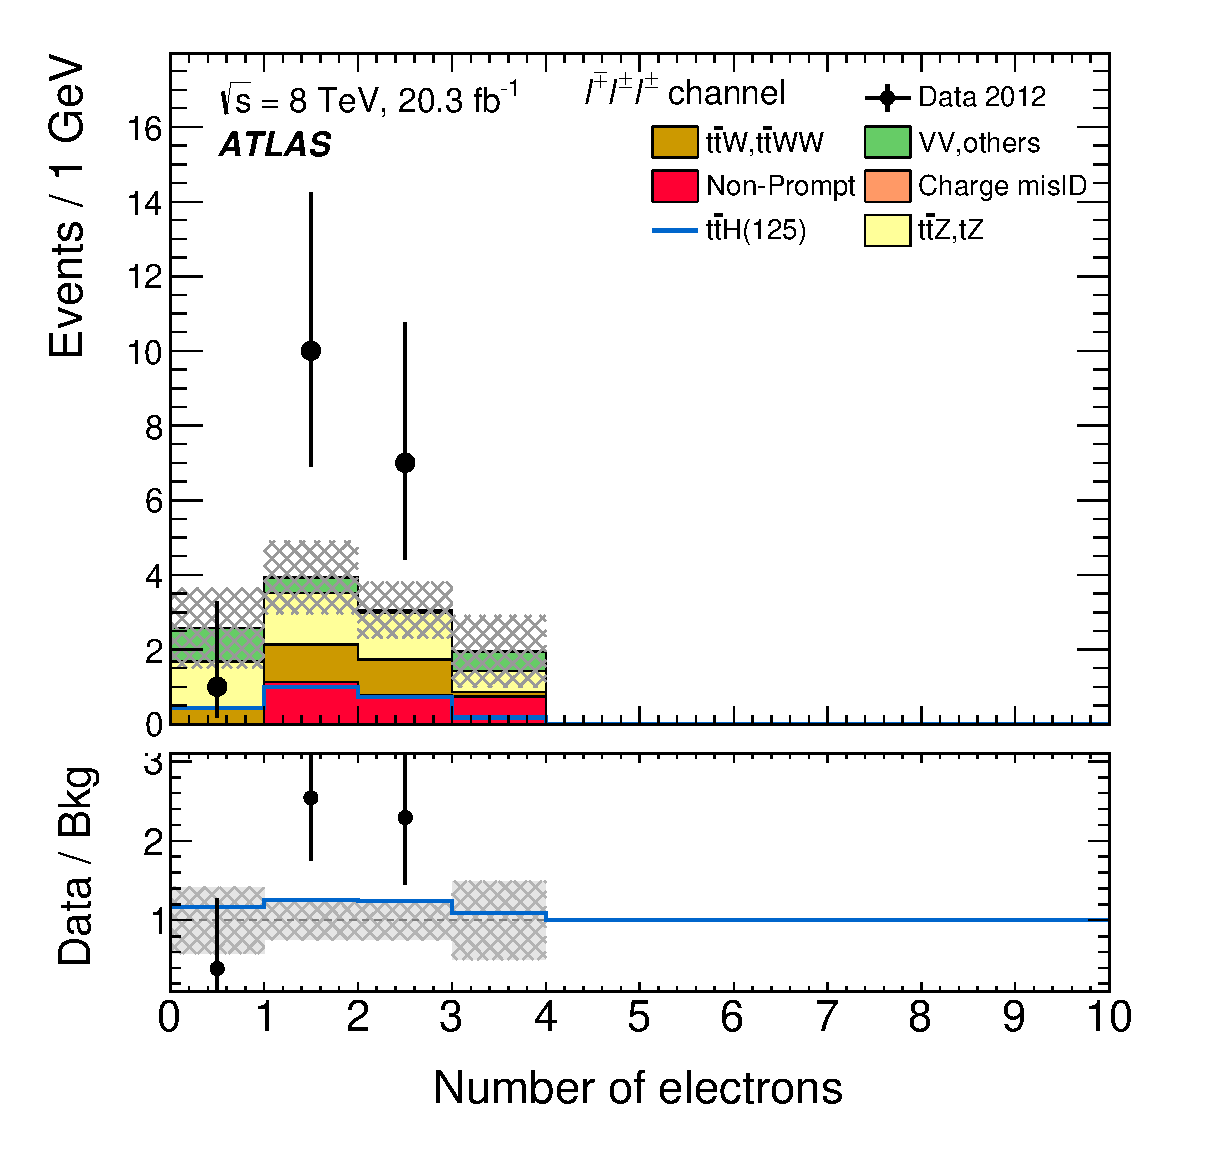
\includegraphics[width=\textwidth]{figs/results/results_new/3lep_SR_NElec}
  \end{minipage}\hfill
  \begin{minipage}[h]{0.4\textwidth}
    \centering 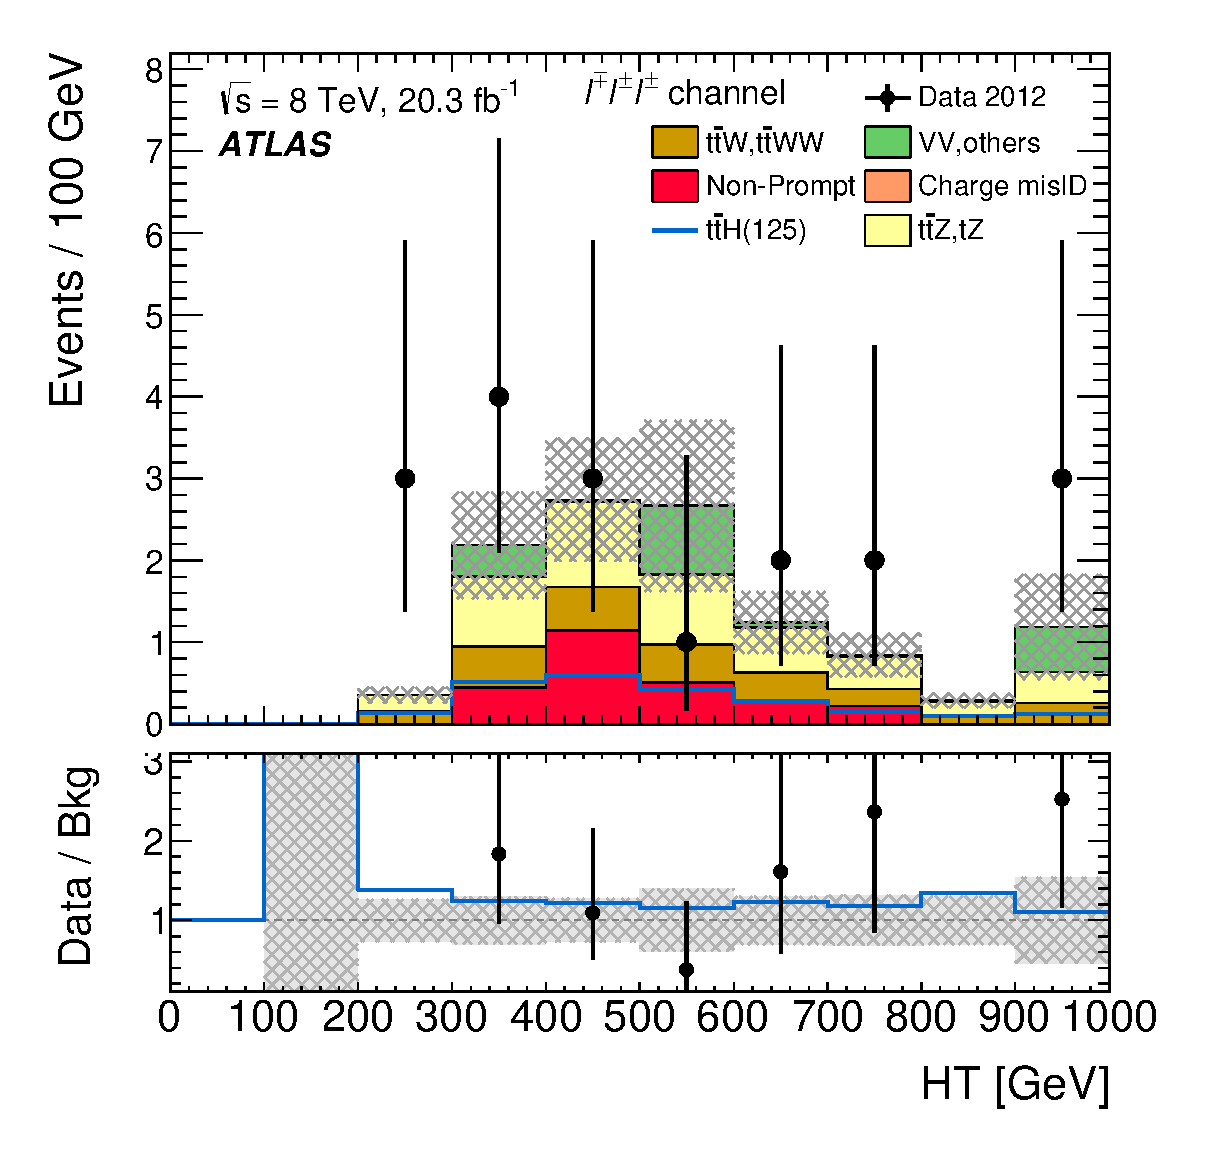
\includegraphics[width=\textwidth]{figs/results/results_new/3lep_SR_HT}
  \end{minipage}\hfill
  \begin{minipage}[h]{0.4\textwidth}
    \centering 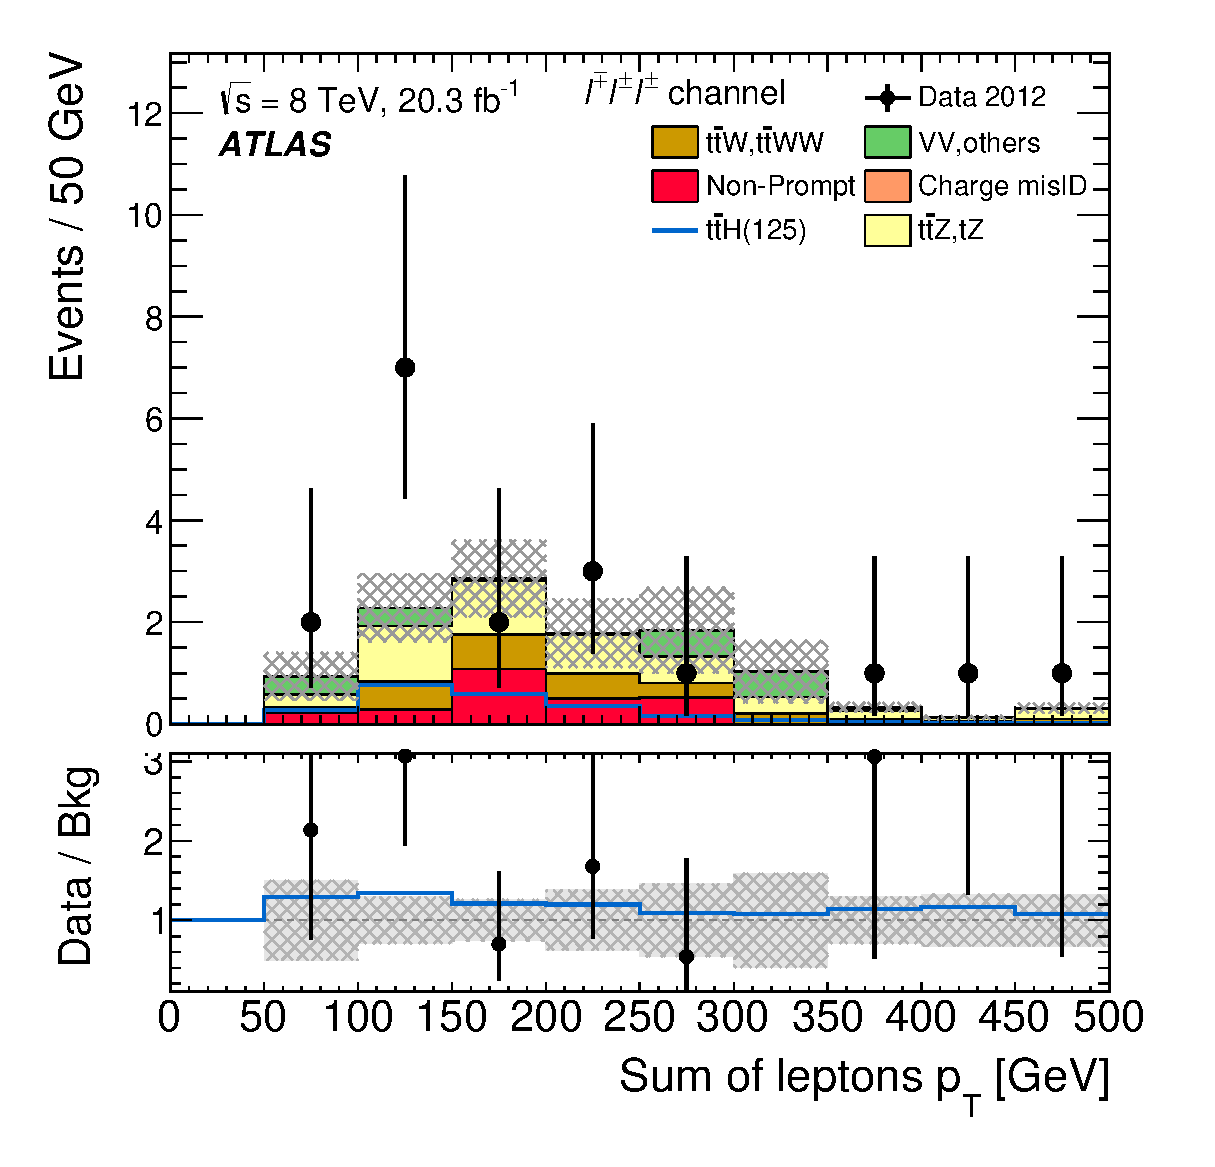
\includegraphics[width=\textwidth]{figs/results/results_new/3lep_SR_SumPtLep}
  \end{minipage}\hfill
  \caption{Jet and b-tagged jet multiplicities (top row);
    10*n(b-tags)+n(jets) and electron multiplicity (middle tow);
    invariant mass of opposite sign lepton pairs; 
    scalar sum of the \pt of selected leptons and jets in the event (bottom left) and only of leptons (bottom right).
}
  \label{figure:results_3l_event}
\end{figure} 
%
\begin{figure}[!htbp]
  \begin{minipage}[h]{0.4\textwidth}
    \centering 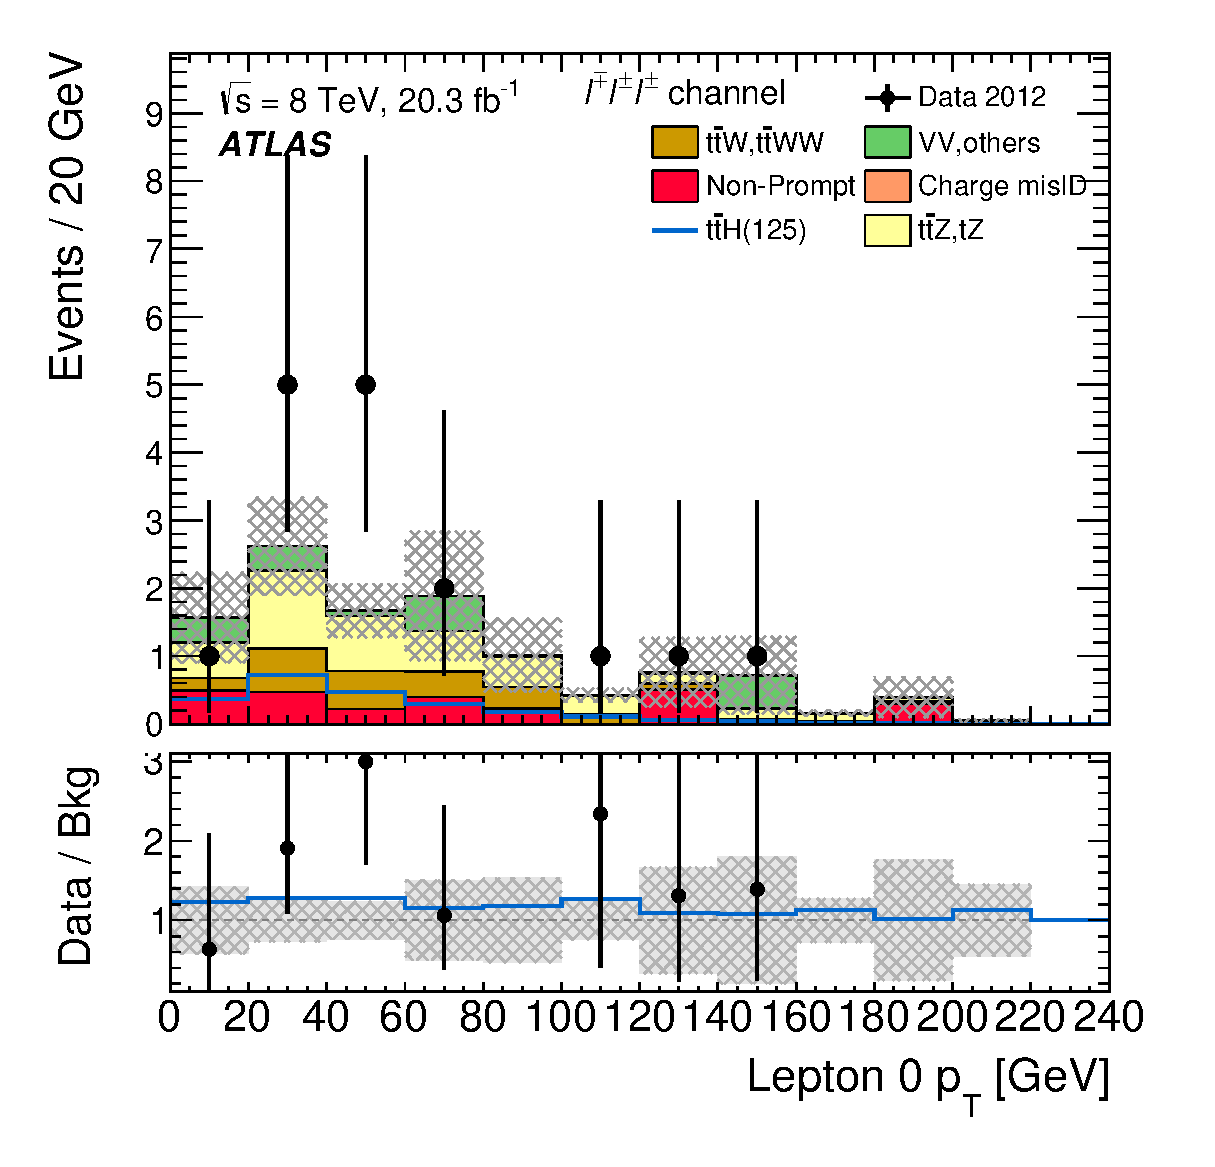
\includegraphics[width=\textwidth]{figs/results/results_new/3lep_SR_SortLep0Pt}
  \end{minipage}\hfill
  \begin{minipage}[h]{0.4\textwidth}
    \centering 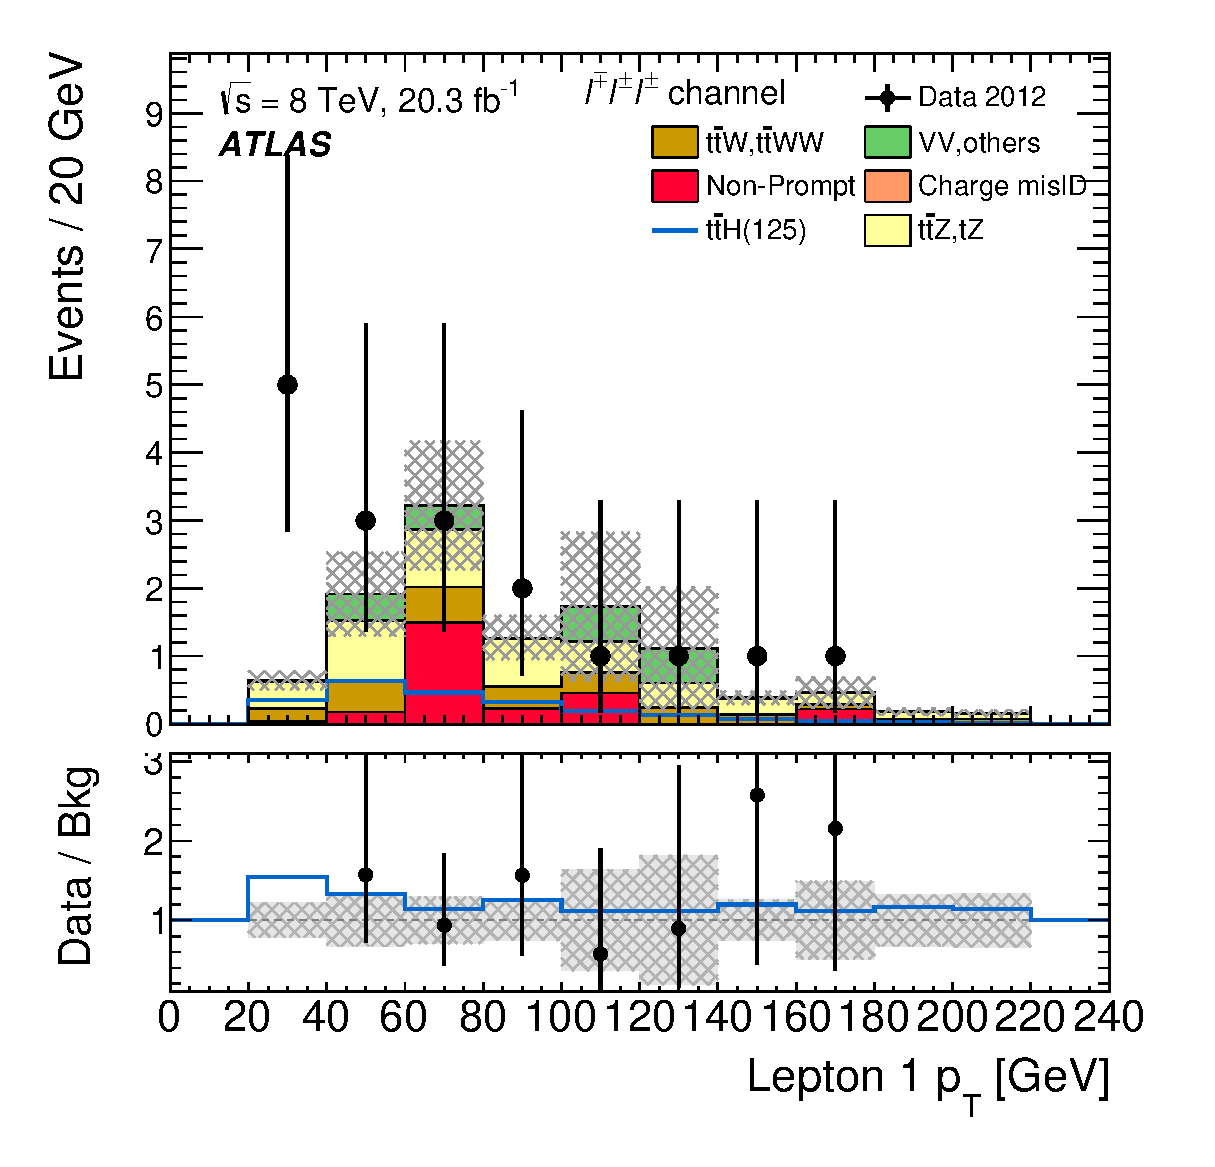
\includegraphics[width=\textwidth]{figs/results/results_new/3lep_SR_SortLep1Pt}
  \end{minipage}\hfill
  \begin{minipage}[h]{0.4\textwidth}
    \centering 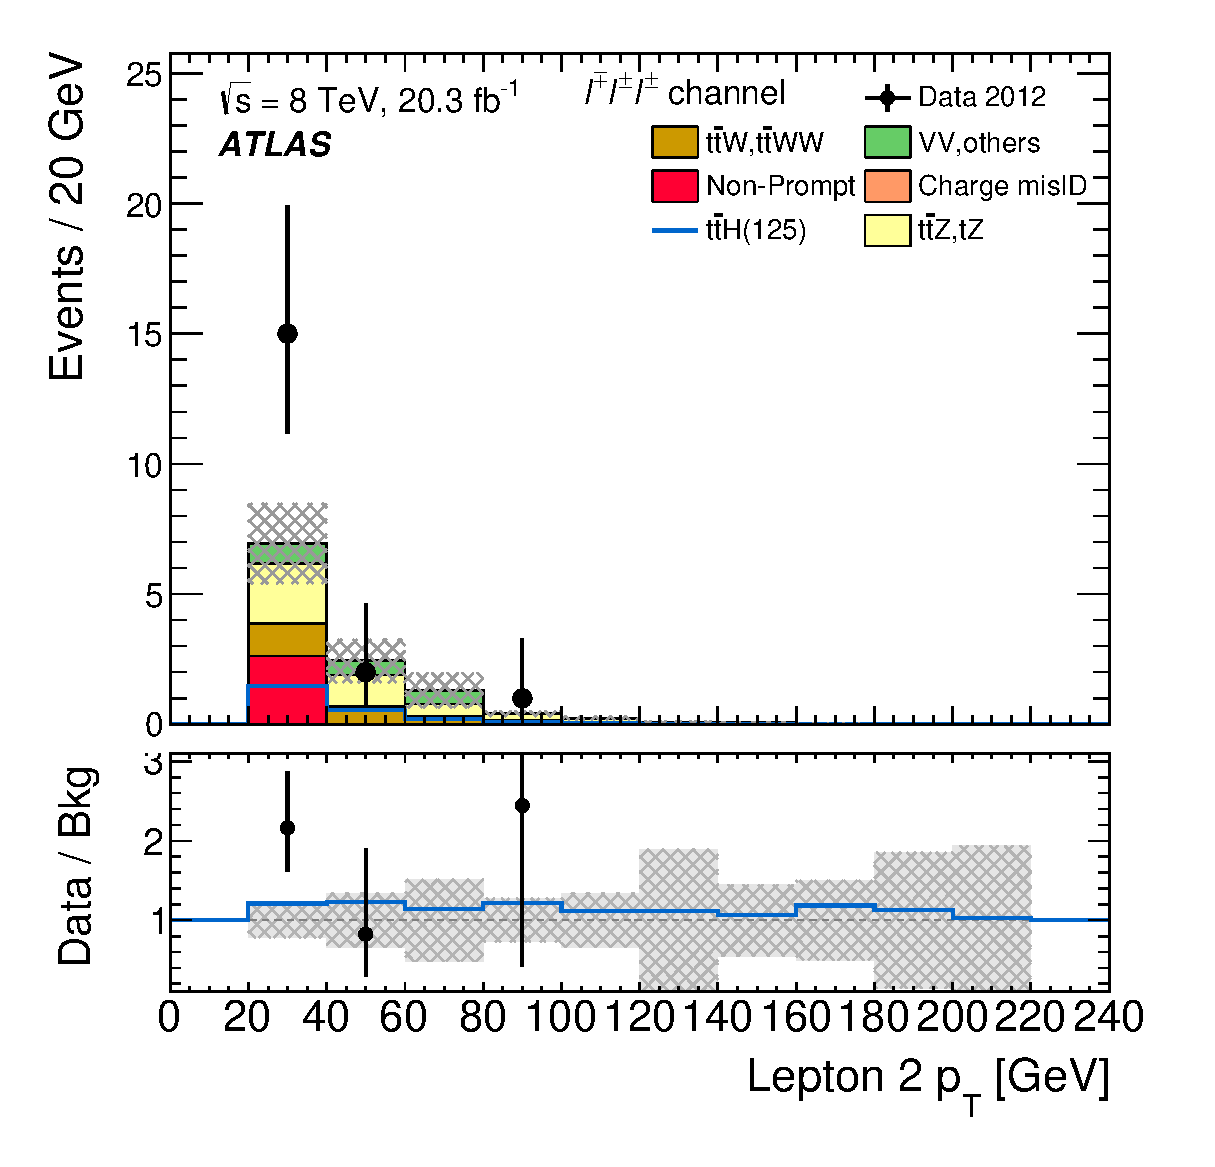
\includegraphics[width=\textwidth]{figs/results/results_new/3lep_SR_SortLep2Pt}
  \end{minipage}\hfill
  \begin{minipage}[h]{0.4\textwidth}
    \centering 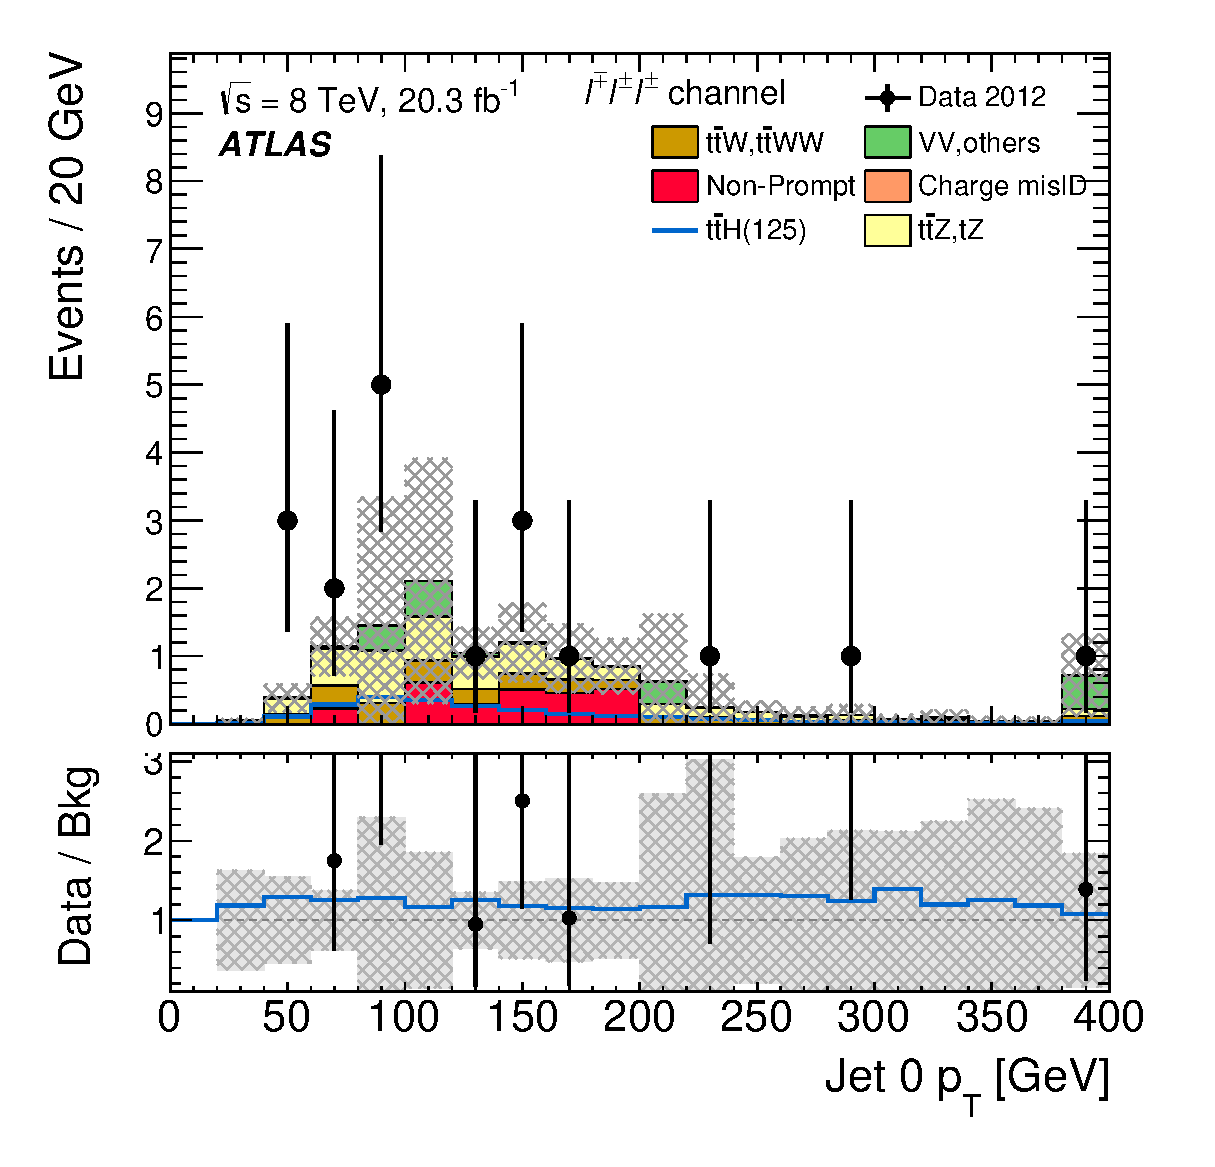
\includegraphics[width=\textwidth]{figs/results/results_new/3lep_SR_jet00_Pt}
  \end{minipage}\hfill
  \begin{minipage}[h]{0.4\textwidth}
    \centering 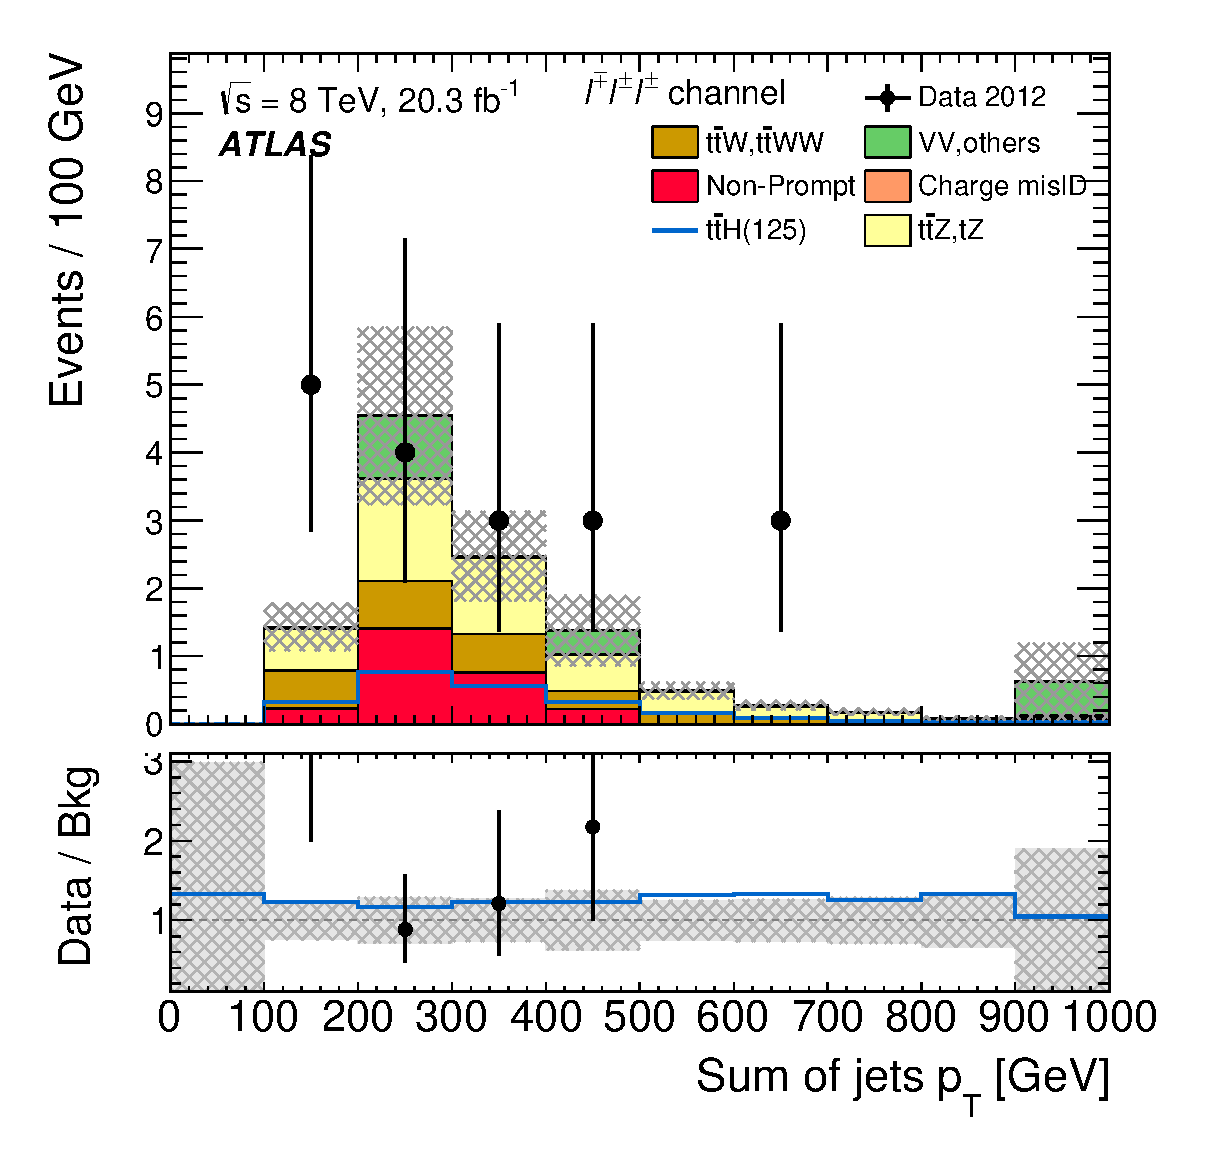
\includegraphics[width=\textwidth]{figs/results/results_new/3lep_SR_SumPtJet}
  \end{minipage}\hfill
  \begin{minipage}[h]{0.4\textwidth}
    \centering 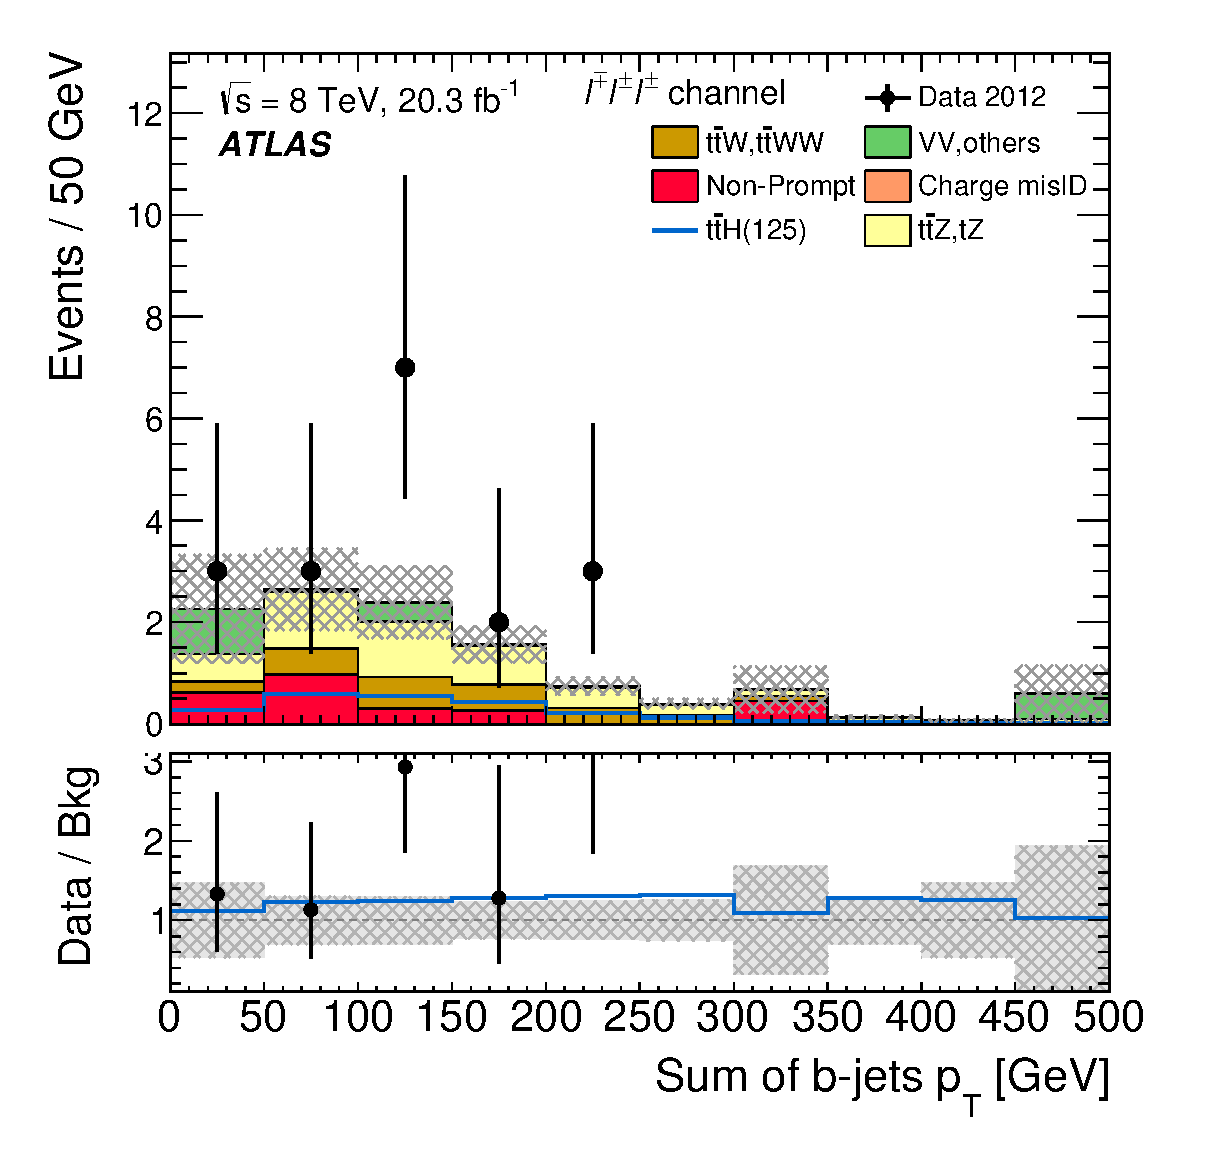
\includegraphics[width=\textwidth]{figs/results/results_new/3lep_SR_SumPtBJet}
  \end{minipage}\hfill
  \caption{Lepton 0 \pt (top left) and lepton 1 \pt (top right); 
    lepton 2 \pt (middle left) and leading jet \pt (middle right); 
    scalar sum of the \pt of selected jets in the event (bottom left) and only of b-tagged jets (bottom right).
    Lepton 0 is the one with opposite charge with respect to lepton 1 and 2, where lepton 2 has lower $\pT$ than lepton 1.}
  \label{figure:results_3l_jet}
\end{figure} 
\begin{figure}[!htbp]
  \begin{minipage}[h]{0.4\textwidth}
    \centering 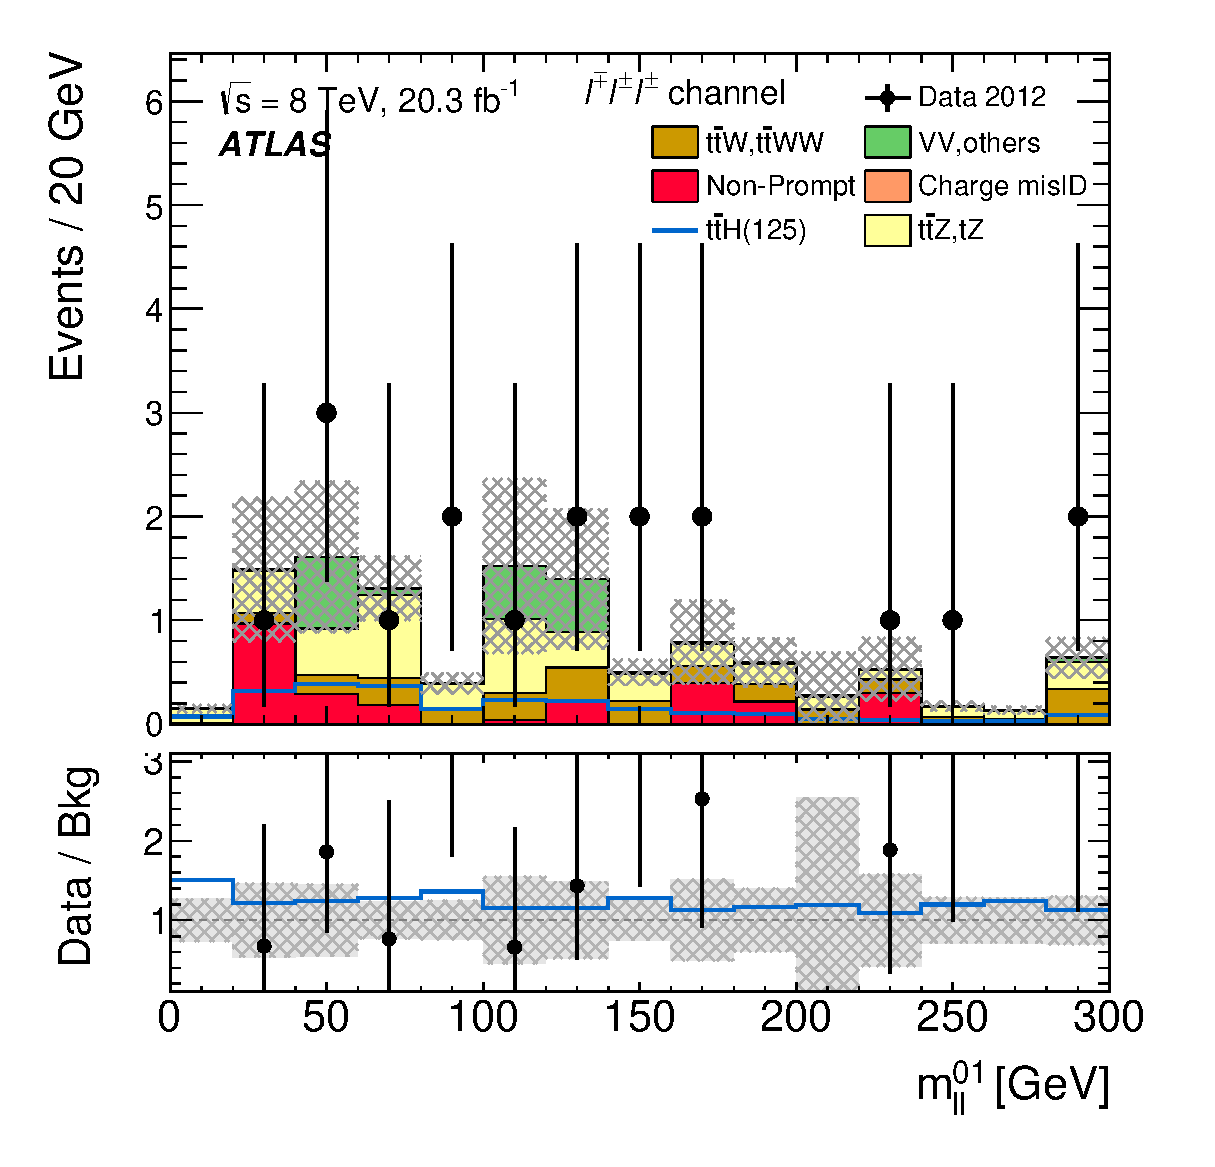
\includegraphics[width=\textwidth]{figs/results/results_new/3lep_SR_SortLepPair01Mll}
  \end{minipage}\hfill
  \begin{minipage}[h]{0.4\textwidth}
    \centering 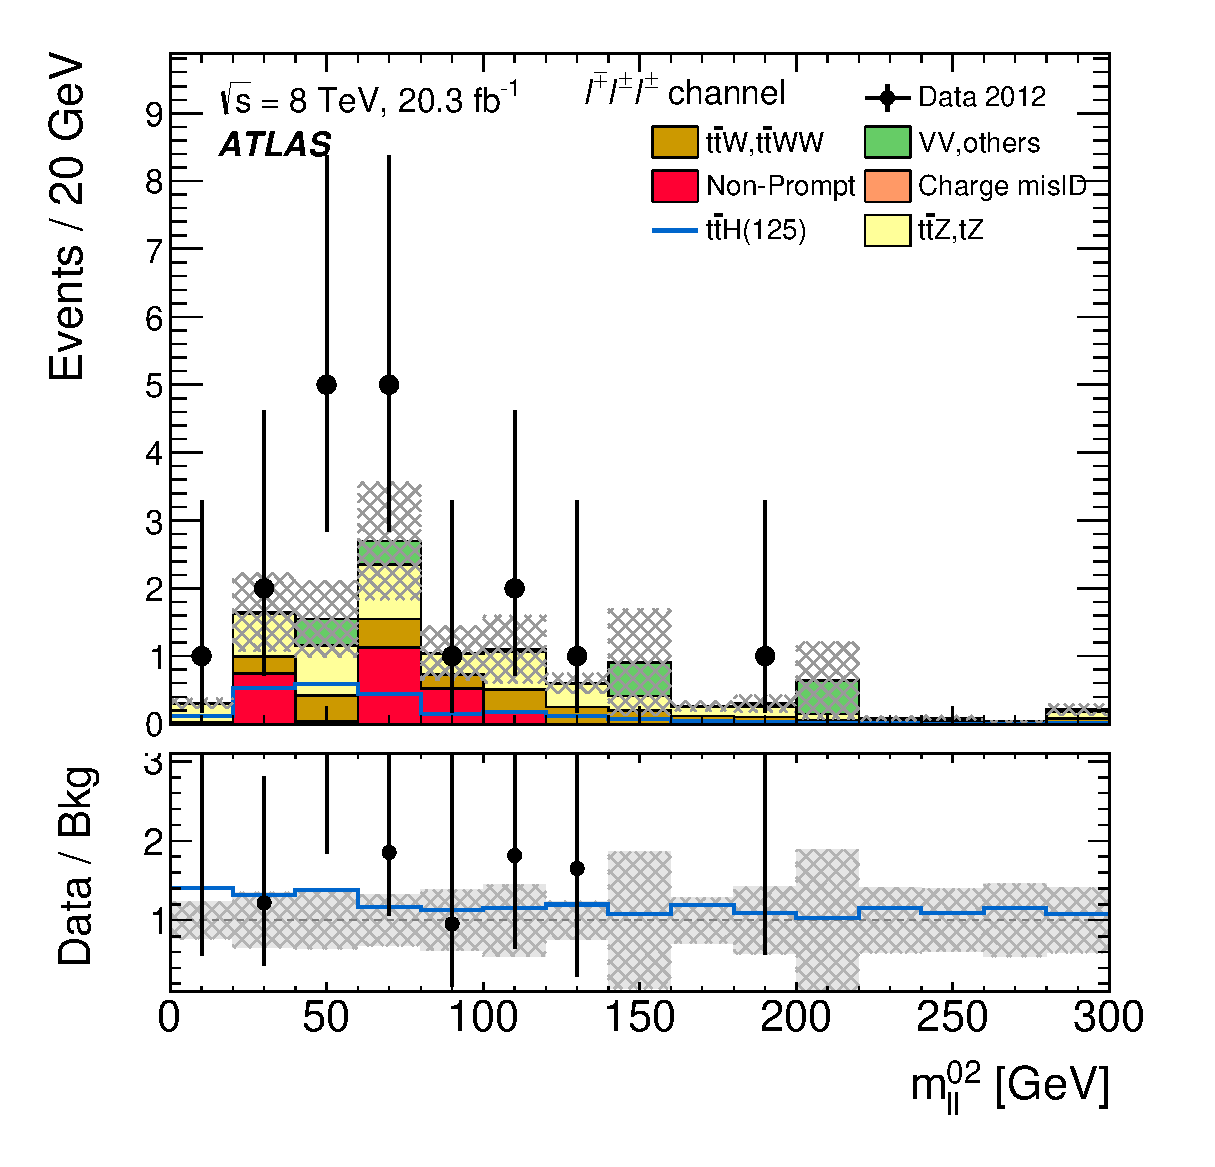
\includegraphics[width=\textwidth]{figs/results/results_new/3lep_SR_SortLepPair02Mll}
  \end{minipage}\hfill
  \begin{minipage}[h]{0.4\textwidth}
    \centering 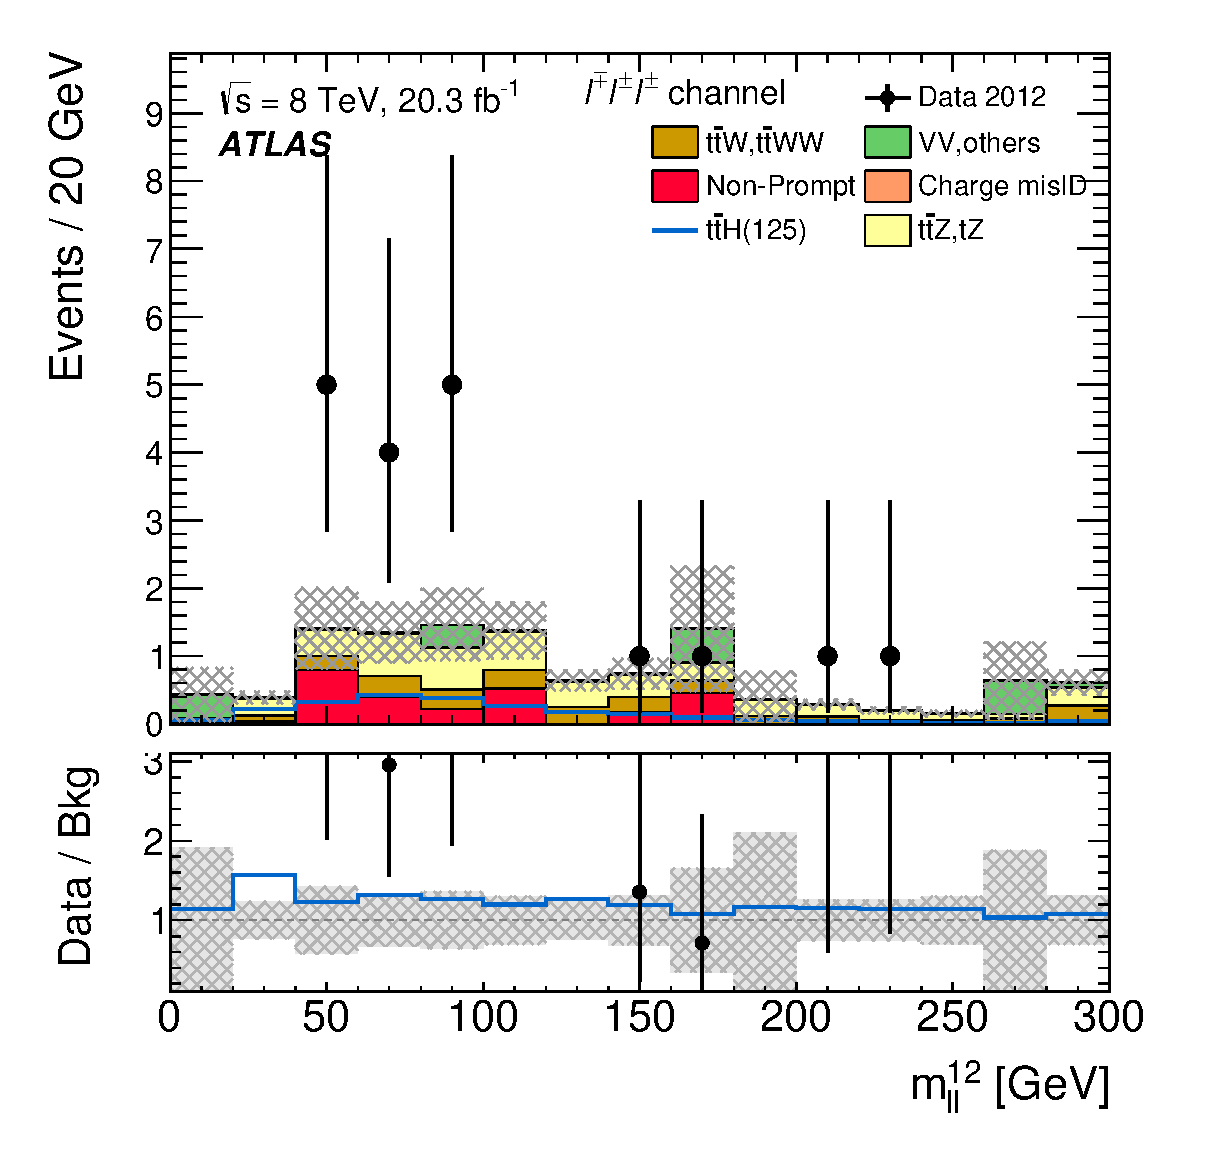
\includegraphics[width=\textwidth]{figs/results/results_new/3lep_SR_SortLepPair12Mll}
  \end{minipage}\hfill
  \begin{minipage}[h]{0.4\textwidth}
    \centering 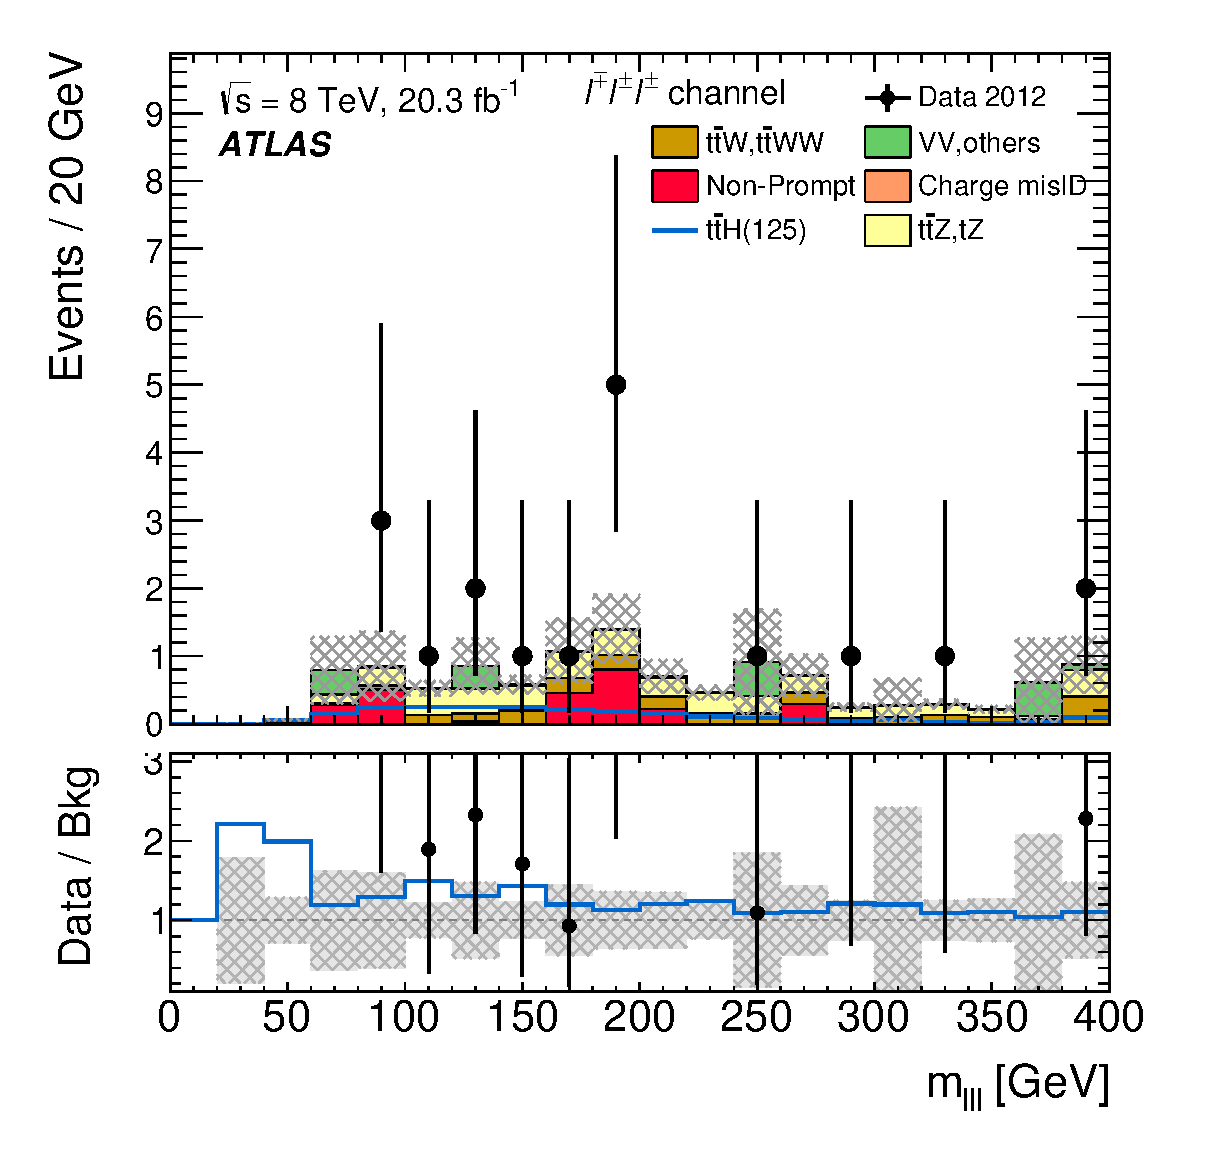
\includegraphics[width=\textwidth]{figs/results/results_new/3lep_SR_Mlll}
  \end{minipage}\hfill
  \caption{Invariant mass of opposite sign lepton pairs (top); (bottom row) invariant mass
    of the three lepton system in the inclusive $WZ$ VR. 
}
  \label{fig:SR3l_mll}
\end{figure} 



\section{Statistical Model}

We use the above results to make two sets of measurements: an upper confidence limit on $\mu$, the signal strength parameter, and a measurement of $\mu$. These measurements are done for each channel individually and then combined. The interpretation of the results in the form of a statistical model follow the procedure, discussed here \cite{asym}. We interpret the results as counting experiments in each signal region. Therefore agreement in kinematic shapes do not affect the statistical procedure. 


\subsection{The Likelihood} 
The observed and expected event yields in the signal regions are analyzed using a binned likelihood function ($\mathcal{L}$), built from product of Poisson models of expected event counts for each bin, where the bins are the separate signal regions:
\begin{equation}
\mathcal{L}\ \alpha\  \prod_{i=0}^{N_{SR}} P(N_{obs}^{i}| \mu \cdot s_{exp}^{i} + b_{exp}^{i})
\end{equation}
where $s_{exp}^i$ is the SM signal expectation in the signal region, $b_{exp}^i$ are the background expectations, $i$ counts over the signal regions, and P is the Poisson distribution. The signal strength parameter is the parameter of interest in the model (POI) and acts as a simple scale-factor to the SM \tth production rate and is common to all channels. Setting $\mu$ to 0 corresponds to the background only scenario. The background parameter, $b$, is a sum over all background processes. 

The signal and background expectations, $s$ and $b$, depend on systematic errors. These are included in the likelihood function in the form of a vector nuisance parameters, $\vec{\theta}$, which are constrained to fluctuate within Gaussian distributions. These fluctuations affect the background and signal expectations by response functions, $\nu(\vec{\theta})$, set by systematic uncertainties measured in the previous section. For instance, the \WZ normalization uncertainty is 50\% from Section~\ref{section:wz} and is included in the fit as its own unit Gaussian,$G(\theta|0,1)$. The fluctuations of the Gaussian, $\theta_{WZ}$, scale the background contribution via the form, $0.5\cdot(1+\theta_{WZ})\cdot b_{WZ}$. For many of the detector systematics, the uncertainties are two sided and are included as piecewise Gaussians. We add correlations to various uncertainties by hand, when appropriate. With these nuisance parameters, the likelihood takes this form:
\begin{equation}
\mathcal{L}(\mu,\vec{\theta})\ =  \left( \prod_{i=0}^{N{ch}} P(N_{obs}^{i}; \mu \cdot \nu_{s}(\vec{\theta})\cdot s_{exp}^{i} + \nu_{b}(\vec{\theta})\cdot b_{exp}^{i}) \right) \times \prod_{j}^{N_{\theta}}G(\theta_j; 1,0)
\end{equation}


\subsection{Test Statistic and Profile Likelihood}

Values of $\mu$ are tested with the negative log quantity, $q_{\mu}= -2$ln$(\lambda(\mu))$, where $\lambda(\mu)$ is the test statistic.
$\lambda(\mu)$ is defined as:
\begin{equation}
\lambda(\mu) \equiv \frac{\mathcal{L}(\mu,\hat{\vec{\theta_{\mu}}})}{\mathcal{L}(\hat{\mu},\hat{\vec{\theta}})}
\end{equation}
where $\hat{\vec{\theta_{\mu}}}$ are values of the nuisance parameter vector that maximize the likelihood for a given value of $\mu$ and $\hat{\mu}$ and $\hat{\vec{\theta}}$ are the fitted values of signal strength and nuisance parameters that maximize the likelihood overall. $\mu$ is constrained to be positive.  

\subsection{ CL$_{s}$ Method}

Exclusions limits on the signal strength are calculated with the test statistic using a modified frequentist method, called the CL$_{s}$ method\cite{0954-3899-28-10-313}. CL$_{s}$ is defined as a ratio of two frequentist quantities. The numerator quantifies the probability of finding the observed data given the signal $+$ background hypothesis. The denominator quantifies the probability of the data given the background only hypothesis.

Using the numerator alone has the undesirable property that, if the data fluctuates below the expectation, an exclusion limit can be reached that is far beyond the sensitivity of the experiment. Normalizing to the background only hypothesis penalizes these low sensitivity cases.

The probability of obtaining an observation as extreme as the data given a particular signal $+$ background hypothesis is given by the p-value, $p_{\mu}$ defined as:
\begin{equation}
 p_{\mu} = \int_{q_{\mu}^{obs}}^{\infty} f(q_{\mu}) dq_{\mu}
\end{equation}
, and the probability of obtaining an observation as extreme as the data given the background hypothesis, $p_b$ is:
\begin{equation}
 p_{b} = \int_{q_{\mu=0}^{obs}}^{\infty} f(q_{\mu=0}) dq_{\mu=0}
\end{equation}
, where $f(q_{\mu})$ is the distribution of $q_{\mu}$ for all possible observations for a given $\mu$ and $q$ is defined above. Therefore,
\begin{equation}
 CL_{s} = \frac{p_{\mu}}{1-p_b}
\end{equation}
A $\mu$ value is considered excluded at 95\% confidence when CL$_{s}$ is less than 5\%. 

\subsection{Exclusion Limits}

Figure~\ref{figure:results_limits} and table \ref{table:limits} show the expected and observed exclusion limits for all channels.


\begin{table}[h!]
\centering
\caption{Expected and observed 95\% CL$_s$ limits on $\mu$ for the combined and split signal regions}
\begin{tabular}{|c|c|c|c|}
\hline
& Expected Limit & Expected SM Signal Injected Limit  & Observed Limit\\ 
\hline
\textbf{Combined} & 2.55& 3.42& 5.50\\
\hline 
\textbf{2$\ell$ SS} & 3.58 &4.51 & 6.50 \\  
\hline
2$\ell$ee &8.95 &9.81 &12.62\\   
2$\ell$em &4.89 &5.82 &7.84\\
2$\ell$mm &5.30 &6.22 &8.30\\
\hline
\textbf{3$\ell$}  &3.67 &4.65 &6.86\\  
\hline
\textbf{4$\ell$}  &14.89 &16.45 &18.05\\  
\hline
\end{tabular}
\label{table:limits}
\end{table}

\begin{figure}[htbp]
\begin{center}
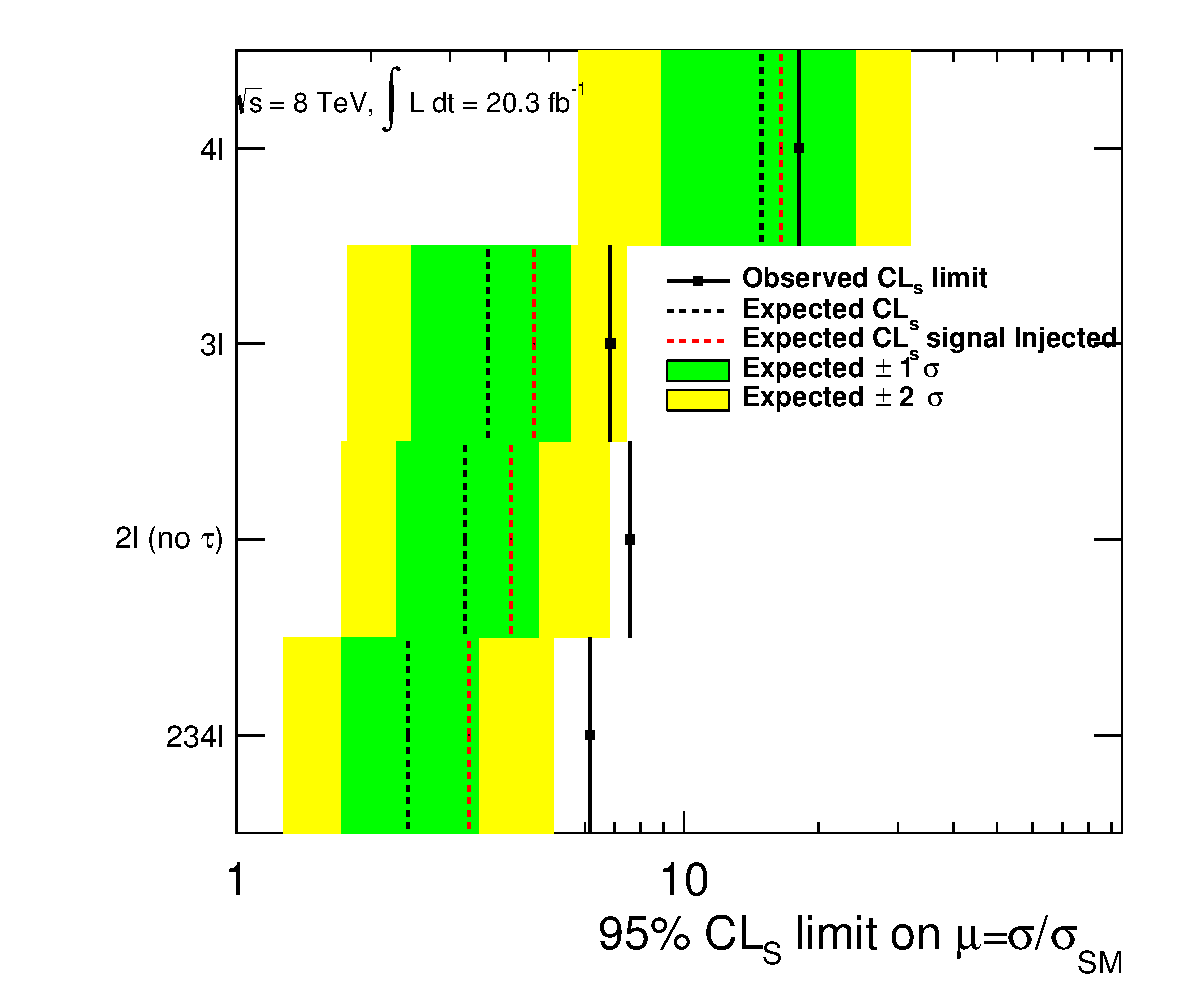
\includegraphics[width=0.7\textwidth]{figs/results/Limits_Obs.pdf}
\caption{Plot of the 2$\ell$ SS, 3$\ell$, 4$\ell$, and combined 95\% CL$_{s}$ observed limits on $\mu$. The expected 1-$\sigma$ (green) and 2-$\sigma$ (yellow) error bands are shown around
the expected limit. The expected limit with SM signal injection ($\mu=1$) is included as well.}
\label{figure:results_limits}
\end{center}
\end{figure}



\subsection{$\mu$ Measurement}

In addition to setting a limit on the signal strength, we also fit the best value of the signal strength for $\mu$. We do this by minimizing the negative log likelihood value, $q_{\mu}$ or conversely maximizing the likelihood. The 1-$\sigma$ error band is set via a profile likelihood scan, where the value $q_{\mu}$ is scanned as a function of $\mu$. Values of $\mu$ that increase $q^{min}_{\mu}$ by 1 form the edges of the error band. The fitted value of $\mu$ for all channels separately and combined is shown in Figure~\ref{Tab:MeasuredMu}. The overally uncertainty derives almost equally from statistical and sysetematic uncertainties.  

\begin{table}[htbp]
\begin{center}
\begin{tabular}{|c|c|c|c|c|c|}
\hline
\multicolumn{2}{|c|}{ Channels} &  $\mu$ value &  stat &  syst &  tot \\
\hline 
          &   &  &   &  &    \\
2l     & 2lee   & 3.74 & $^{+3.89}_{-3.25}$ & $^{+2.72}_{-2.44}$ &  $^{+4.75}_{-4.06}$ \\ 
          &   &  &   &  &    \\
        & 2lem  & 2.97 & $^{+2.09}_{-1.83}$ & $^{+1.81}_{-1.56}$ &  $^{+2.77}_{-2.41}$ \\ 
          &   &  &   &  &    \\
        & 2lmm &  2.68 & $^{+2.61}_{-2.22}$ & $^{+1.85}_{-1.48}$ &  $^{+3.20}_{-2.67}$ \\ 
          &   &  &   &  &    \\
        &  All     &2.85 & $^{+1.47}_{-1.35}$ & $^{+1.57}_{-1.28}$ &  $^{+2.15}_{-1.86}$ \\ 
          &   &  &   &  &    \\
\hline 
\cline{1-6} 
\multicolumn{2}{|c|}{  }  &   &   &  & \\
\multicolumn{2}{|c|}{ 3l }  & 2.93 & $^{+1.97}_{-1.68}$ & $^{+0.94}_{-0.62}$ &  $^{+2.19}_{-1.79}$ \\ 
\multicolumn{2}{|c|}{  }  &   &   &  & \\
\hline 
\multicolumn{2}{|c|}{  }  &   &   &  & \\
\multicolumn{2}{|c|}{ 4l }  &1.83 & $^{+6.81}_{0.00}$ & $^{+1.18}_{-0.00}$ &  $^{+6.91}_{0.00}$ \\ 
\multicolumn{2}{|c|}{  }  &   &   &  & \\
\hline 
\multicolumn{2}{|c|}{  }  &   &   &  & \\
\multicolumn{2}{|c|}{ 234l }  & 2.83 & $^{+1.15}_{-1.06}$ & $^{+1.08}_{-0.84}$ &  $^{+1.58}_{-1.35}$ \\ 
\multicolumn{2}{|c|}{  }  &   &   &  & \\
\hline 
\end{tabular} 
\caption{\label{Tab:MeasuredMu}  $\mu$ measurement for all channels and their combination, with asymmetric minos errors. Statistical, systematics and total error are provided. Results are given on a fit to data for all channels.}
\end{center} 
\end{table} 

\subsection{Nuisance Parameter Impact on the Signal Strength}

Finally, we examine the post-fit impact of the various nuisance parameters in Figure~\ref{figure:results_nuisance}.  The fake nuisance parameters are divided for 2$\ell$ into the systematic uncertainty on the transfer factors for electrons and muons (alpha\_Theta\_mm, alpha\_Theta\_ee) and the systematic uncertainties on the number of events in the anti-tight control regions (e.g alpha\_Fakes\_2lem5j). The 3$\ell$ fake uncertainties are contained in a single parameter (alpha\_Fakes\_3l). The theory cross-section (XS) uncertainties are divided into PDF and scale nuisance parameters separately for each background (\ttW,\ttZ,\tth). The most important nuisance parameters associated with the detector and experimental uncertainties are the JES, the b-tag scale-factor weights, and the lepton isolation.  

We have measured the various analysis uncertainties well and do not expect the fit to have much further constraint. For that reason, we expect the pulls of the nuisance parameters to be close to 0 and the measured uncertainties on those parameters to be consistent with the input uncertainties. This is true for all but the 4$\ell$ fake transfer factor which is pulled slightly high by the excess in the $\mu$ channels. The pull is well within the uncertainty. The uncertainties that dominate this fit are those associated with the \ttV\ cross-section and the fake estimates. 

\begin{figure}[htbp]
\begin{center}
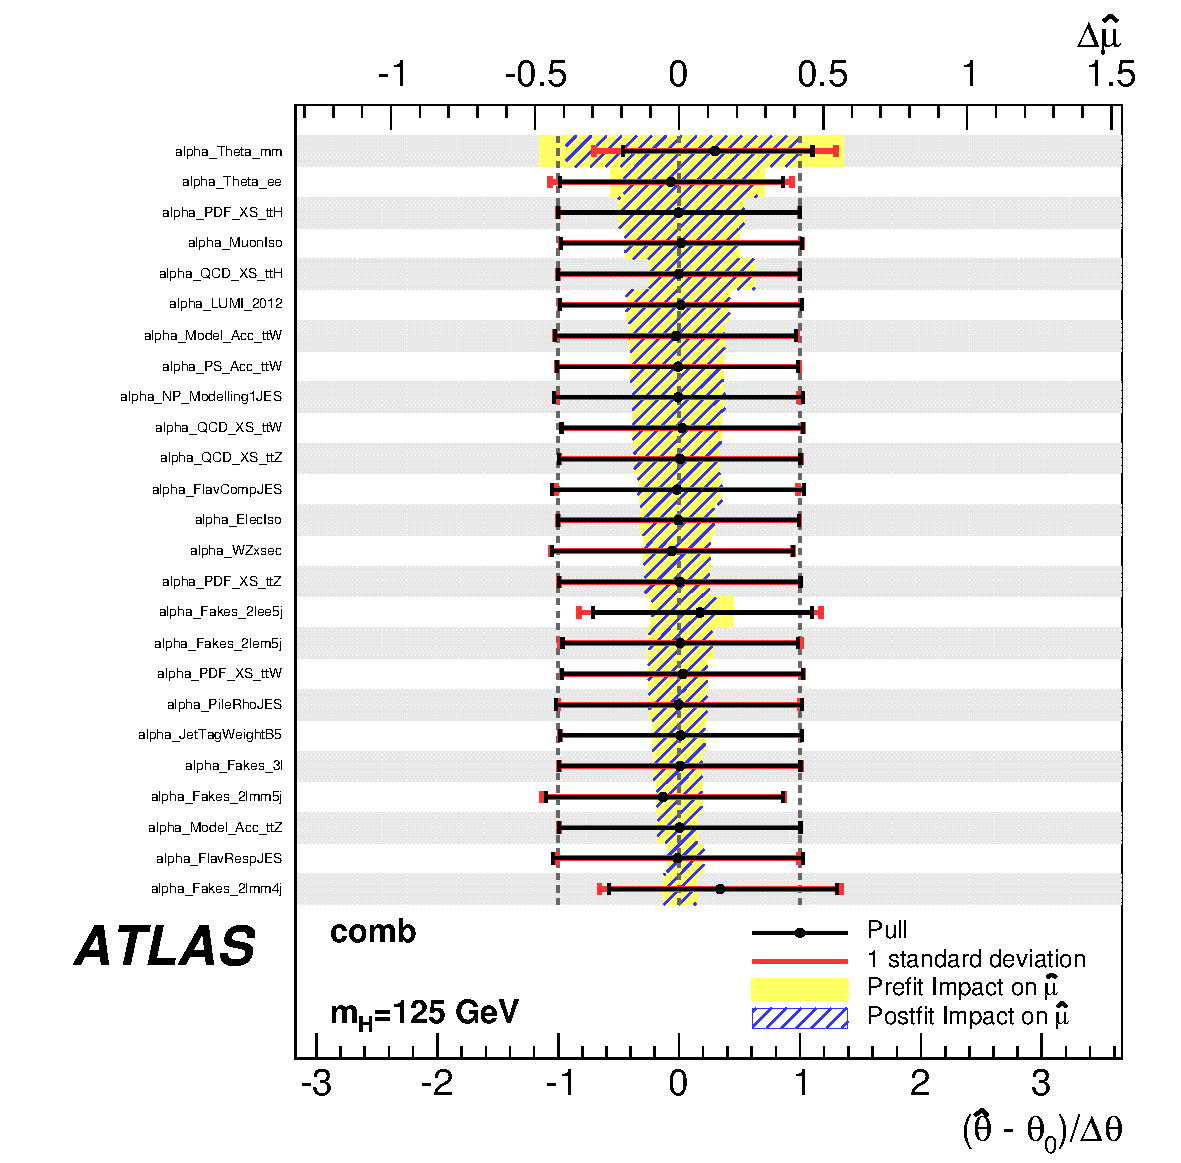
\includegraphics[width=0.7\textwidth]{figs/results/nuisance.pdf}
\caption{Figure of the post- and pre-fit impacts of the top nuisance parameters on the combined $\mu$ measurements}
\label{figure:results_nuisance}
\end{center}
\end{figure}



\section{Discussion of Results and Significance of the Excess}

The results show an overall excess of events over the background-only hypothesis. An excess is observed in both the 2$\ell$ and 3$\ell$ channels. However, the excess is not a considered signficant enough to warrant an observation of new physics.  

A first suspicion would be that two domianant backgrounds are not well modeled: \ttV\ and fake. The fake backgrounds from top have been validated in low jet control regions, and the extrapolation to higher number of jets is constrained by simulation. The anti-tight control regions, shown in Chapter~\ref{chapter:background}, which are enriched in fake events do not show a similar shape to the excesses in the tight signal regions. The \ttV\ cross-section is constrained only by theoretical methods and the \ttZ\ validation region used does show an excess of data events. A rescaling of the \ttV\ by the data/MC ratio show in the \ttZ\ validation regions would not explain the size or shape of the excess, though the significance of the excess would decrease. The \ttZ\ validation region excess is compatible with a statistical fluctuation of the backgrounds, as discussed in Section~\ref{section:ttV}. Indeed, an public ATLAS measurement of the \ttZ\ rate in this 3$\ell$ region shows a deficit of events \cite{ATLAS-CONF-2012-126} using the same MC models. It is therefore not clear that re-scaling the the \ttV\ cross-section is warranted. 

The overall excess of events has peculiar properties: it is found predominantly in events with a large-number of jets and b-tagged jets.  For the 2$\ell$ channel, the excess is found primarily in the $\mu\mu$ and $e-\mu$ flavor bins. Events with large numbers of b-tagged jets and flavor asymmetry are difficult to describe with the standard model backgrounds, even including a standard model Higgs hypothesis. The high \pt\ scale of the excess for sub-leading leptons suggest that the fakes are well understood and the agreement in the 1 b-tagged jet bin suggest that the combined \ttV\ and fakes are under control. 


